\documentclass[a4paper]{report}

\usepackage[top=3cm, bottom=3cm, left=3cm, right=3cm]{geometry}

\usepackage{hyperref}
\usepackage{url}
\usepackage{cite}

\usepackage[usenames,dvipsnames]{xcolor}


\usepackage{tikz}
\tikzset{
  box/.style={
    minimum width=\pagewidth,
    draw,
    rounded corners,
    rectangle
  },
}
\usetikzlibrary{shapes,snakes}
\usepackage{amsmath,amssymb}

\usepackage{float}
\usepackage{wrapfig}

\usepackage[english]{babel}
\usepackage{array}
\usepackage{caption}
\usepackage{subcaption}
\usepackage{graphicx}
\usepackage{sidecap}
\usepackage{float}
\usepackage{varwidth}



% section wise numbering of figures etc..
\usepackage{chngcntr}
\counterwithin{table}{section}
\counterwithin{figure}{section}


\usepackage{ifthen,version}
\newboolean{include-notes}

% commenting...
 \setboolean{include-notes}{true}
\newcommand{\chrisnote}[1]{\ifthenelse{\boolean{include-notes}}%
 {\textcolor{BrickRed}{\textbf{Chris: #1}}}{}}


% for nice warning symbol
%\usepackage{fourier}

% nice circled numbering
\newcommand*\circled[1]{\tikz[baseline=(char.base)]{
            \node[shape=circle,draw,inner sep=2pt] (char) {#1};}}

\newcommand{\HRule}{\rule{\linewidth}{0.5mm}}
\renewcommand{\thesection}{\thepart \arabic{section}}

\usepackage{pict2e,picture}
\newsavebox\CBox
\newlength\CLength
\def\Circled#1{\sbox\CBox{#1}%
	\ifdim\wd\CBox>\ht\CBox \CLength=\wd\CBox\else\CLength=\ht\CBox\fi
	\makebox[1.2\CLength]{\makebox(0,1.2\CLength){\put(0,0){\circle{1.2\CLength}}}%
	\makebox(0,1.2\CLength){\put(-.5\wd\CBox,0){#1}}}}


\begin{document}

	% Define box and box title style
	\tikzstyle{mybox} = [draw=black, fill=white, thick, rectangle, rounded corners, inner sep=0.4cm]
	\tikzstyle{mytitle} =[fill=black,rectangle, rounded corners, text=white]

	\begin{titlepage}
	\begin{center}
		{ \Large \bfseries How to Create Affordable, Anthropomorphic, Personalized, Light-Weight Prosthetic Hands\\[0.5cm] }
                { \large *George P. Kontoudis, *Minas V. Liarokapis, *Agisilaos G. Zisimatos, *Christoforos I. Mavrogiannis and Kostas J. Kyriakopoulos}

                \vspace{1.4in}

		\fbox{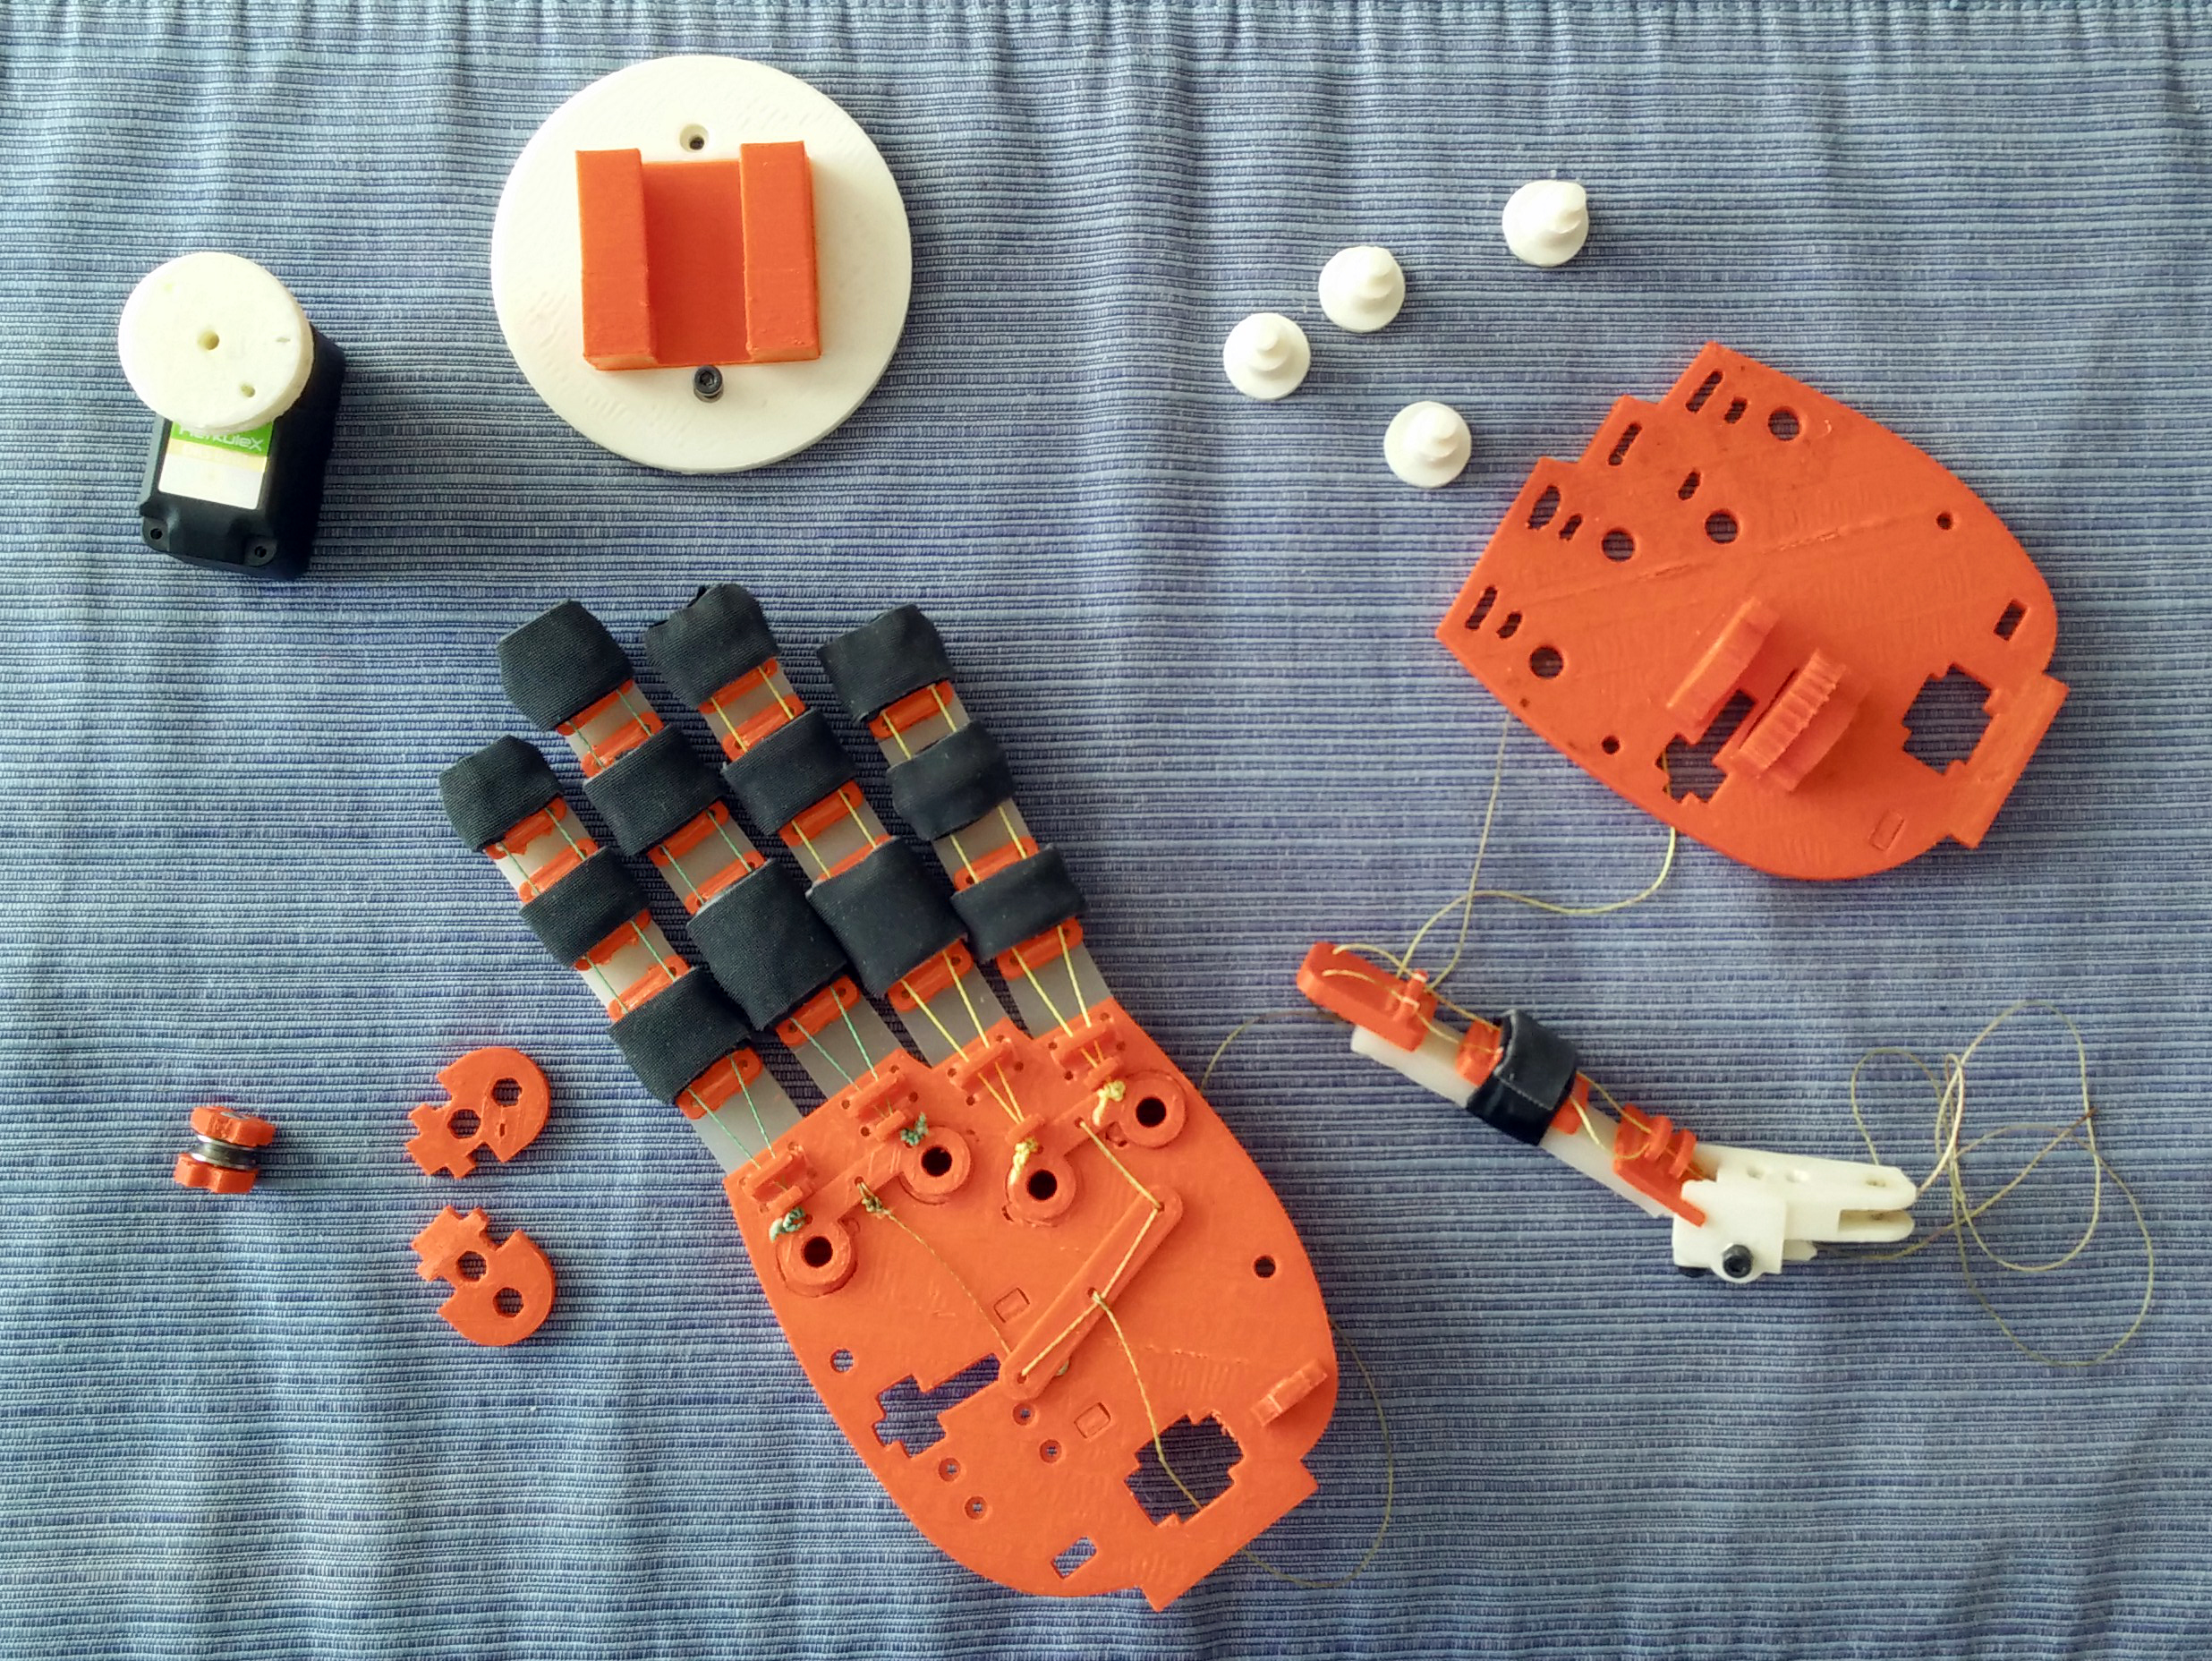
\includegraphics[width=12cm]{figures/cover.jpg}}

                \vspace{1.7in}

		{ \large Technical Report, Control Systems Lab\\
                   School of Mechanical Engineering, National Technical University of Athens \\[0.5cm] }

		{ \large October 2015 $|$ * denotes first author\\[0.5cm]}
		
		
	\end{center}
	\end{titlepage}

	\newpage


	\begin{minipage}{0.2\textwidth}
		
\includegraphics[width=2cm]{figures/License.png}
	\end{minipage}
	\begin{minipage}{0.8\textwidth}
		\begin{flushleft} \small        
			OpenBionics by \url{www.openbionics.org} is licensed under a  \href{https://creativecommons.org/licenses/by-sa/4.0/}{Creative Commons Attribution-ShareAlike 4.0 International License}.
		\end{flushleft}
	\end{minipage}

	\vspace{12cm}

\begin{center}
 
\includegraphics[width=8cm]{figures/openbionics.png}
\end{center}

	{\Large \bfseries Contact: }\\

        \noindent George P. Kontoudis, Agisilaos G. Zisimatos and Kostas J. Kyriakopoulos are with the Control Systems Lab, School of Mechanical Engineering, National Technical University of Athens, 9 Heroon Polytechniou Str, Athens, 15780, Greece (email:\{mc11681,el08087,kkyria\}@mail.ntua.gr).\\

        \noindent Minas V. Liarokapis is with the Dept. of Mechanical Engineering and Materials Science, School of Engineering and Applied Science, Yale University, 9 Hillhouse Avenue, New Haven, CT, 06520, USA (email:minas.liarokapis@yale.edu).\\

        \noindent Christoforos I. Mavrogiannis is with the Sibley School of Mechanical \& Aerospace Engineering, Cornell University, Ithaca, NY, 14853, USA (email:cm694@cornell.edu).\\

	\noindent For any inquiry and/or suggestion you may contact: info@openbionics.org 
	

\newpage
\tableofcontents
\newpage
\section{Introduction}


\indent This technical report is intended to serve as a step by step tutorial for the replication of a prosthetic hand \cite{Kontoudis2015IROS} developed by the \href{www.openbionics.org}{OpenBionics (www.openbionics.org)} initiative \cite{Liarokapis2014ASURRW}. Based on a previous design for the OpenBionics robotic hands \cite{Zisimatos2014IROS}, the prosthetic hand was developed to be affordable, light-weight and intrinsically-compliant. The proposed design is also structurally and kinematically anthropomorphic. In particular, its sizing is parametrically determined in an anthropomorphic fashion, according to data provided by hand anthropometry studies \cite{BuchholzErgonomics1992}, allowing for personalization and adjustment to the needs of each individual. Moreover, its kinematic model is derived by incorporating an index of Anthropomorphism \cite{Liarokapis2013ICRA} in the design optimization process. Finally, the prosthetic hand bears a novel differential mechanism based on the \textit{whiffletree} or \textit{seesaw} mechanism that allows the user to switch between various postures using a single actuator. Postures and gestures selection is easy and intuitive, through the use of simple locking buttons that can independently block the motion of each finger. The proposed hands can be easily fabricated using low-cost, off-the-shelf materials and rapid prototyping techniques. 

 
In the following sections, we describe in detail all the necessary steps for the replication of the proposed prosthetic hand. In order to facilitate the fabrication for non-expert users, effort has been devoted to utilize off-the-shelf materials and equipment that can be easily found in hardware stores around the world.

\section{Prosthetic Hand Design}

In this section we present the prosthetic hand design. The hand is underactuated as all five fingers are controlled with a single actuator which is mounted on the palm. The transmission is achieved with tendons driven through low-friction tubes. A differential mechanism facilitates the execution of multiple postures and gestures with the single actuator. 

\subsection{Anthropomorphism}

Recently, Liarokapis et al. \cite{Liarokapis2013ICRA} formalized an index of anthropomorphism for quantifying the humanlikeness of robot hands in terms of motion capabilities and morphology. The index was defined as the weighted sum of workspace similarity subscores. These subscores were derived from comparisons between the robot hand and a human hand reference. Human hand anthropometry studies \cite{BuchholzErgonomics1992} were used to define the representative human hand model. The proposed index of anthropomorphism can be used in order to assess the humanlikeness of existing robot hands, or as an optimization criterion for designing a new generation of robot and prosthetic hands. We argue that anthropomorphism not only results to more aesthetically superior artifacts but also to a better performance in everyday life grasping and manipulation tasks. This conclusion was based on the simple observation that the objects surrounding us have been crafted according to the design and the capabilities of the human hand. Therefore, structurally and kinematically anthropomorphic artificial hands may be more well suited to execute a wide variety of everyday life tasks. 

Based on this observation, we used the index of Anthropomorphism to extract specifications for the design of our anthropomorphic prosthetic hand. In particular, we optimized for anthropomorphism with respect to the finger phalanges lengths and the positions/orientations of the finger base frames. The human hand reference was extracted from parametric models \cite{BuchholzErgonomics1992} that only require two human hand parameters: 1) the hand length (HL) and 2) hand breadth (HB). 

Finally, the extracted finger base frames orientations were further optimized to allow for a satisfactory Kapandji score \cite{Kapandji}. The Kapandji score is a tool that is widely used by physicians in order to evaluate a patient's thumb opposition capability by asking the subject to use their thumb to touch a set of different palm locations. Based on the locations reached, a score indicative of the thumb's opposition dexterity is determined by the Kapandji scale. This tool has lately found applications in robot hand design \cite{GrebensteinThesis}. Inspired by the aforementioned study, we used the Kapandji score as a criterion for determining the hand's kinematics in order for the thumb fingertip to be able to make contact with 1) the base frames of the remaining four fingers and 2) the tips of the index and pinky fingers. 

%\ref{baseFrames}.

%as shown in Fig. \ref{fingertips}.


\subsection{Finger Design}

Each one of the index, middle, ring and pinky fingers consists of three phalanges and three rotational Degrees of Freedom (DoF) for flexion/extension, while the thumb consists of two phalanges and two rotational DoF for flexion/extension and one rotational DoF for abduction/adduction. All joints of the fingers are flexure joints based on elastomer materials (silicone or polyurethane sheets), the sizing of which was determined empirically to achieve both a lightweight structure and a force range that is adequate for everyday life tasks \cite{DollarAR2005}. In terms of functionality, the aforementioned finger actuation and transmission is bioinspired, in the sense that it structurally replicates the flexion/extension motions of the human fingers. More specifically, the use of elastomer materials on the joints implements the passive extension, while cables (Dyneema fishing line) driven through low-friction tubes implement the flexion. Finally, in order to enhance stability through force impact absorption and increased friction at the contacts \cite{deformableciocarlie2005}, we covered the fingertips with: 1) deformable sponge-like tape , 2) rubber tape and 3) anti-slip tape.

\subsection{Palm}

The palm consists of two parallel planes that can be made out of Plexiglas (acrylic) or ABS (depending on the manufacturing technique used) and which  accommodate: 1) the finger base frames, 2) the thumb mechanism, 3) the selectively lockable differential mechanism (i.e., the whiffletree and the buttons) and 4) the actuator base. In the following sections we describe in detail the thumb locking mechanism and the selectively lockable differential mechanism.

  
\subsubsection{Thumb Locking Mechanism}

For the thumb we use a selectively lockable toothed mechanism that can implement 9 different opposition configurations as depicted in Fig. \ref{thumb}. These configurations were selected to allow the efficient execution of the Kapandji test \cite{Kapandji} and to allow also the user to switch among different grasping postures (e.g., pinch grasp, power grasp, key grasp etc.). The proposed one DoF thumb mechanism serves as a simple alternative to the mechanically complex three DoF human thumb. The proposed mechanism is completely stiff when it is locked, in contrast to the friction based mechanisms \cite{Baril} that are affected by torsional forces that are inherent in dynamic/unstructured environments (these forces can result to large, uncontrolled displacements of the thumb for these mechanisms). The thumb tendon is terminated to an appropriate servo pulley. Small motor angular displacements are required for the finger to be actuated. Finally, the diameters of the pulleys were optimized for the Kapandji test \cite{Kapandji}.

\begin{figure}[h]
%\setlength{\belowcaptionskip}{-8pt}
%\setlength{\abovecaptionskip}{-6pt}
\begin{center}
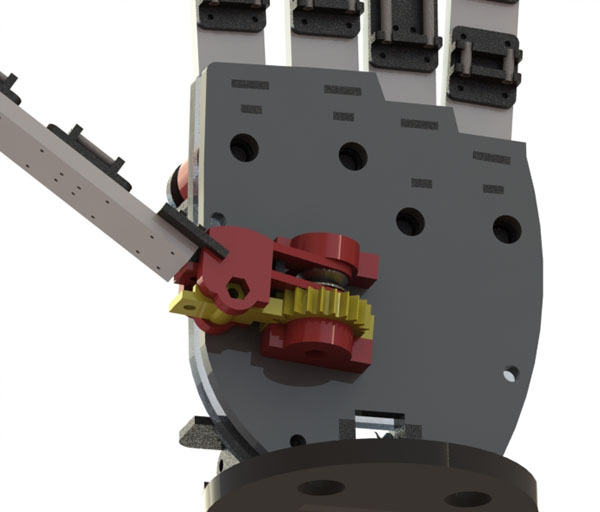
\includegraphics[width=6.4cm]{figures/paper_images/thumbmechanism.jpg}
\end{center}
\caption{The thumb mechanism consists of the red and golden parts. The red parts are mounted in appropriate slots on the robot palm to facilitate installation of the thumb mechanism. The golden parts are: 1) a pulley that routes the thumb tendon to the back of the hand and 2) the toothed, selectively lockable mechanism that allows adjustment of thumb's opposition. The robot thumb can be passively positioned by the user, in 9 discrete configurations.} 
\label{thumb}
\end{figure}

\subsubsection{A Selectively Lockable Differential Mechanism}

A selectively lockable differential mechanism connects the actuator with the tendons of each finger. The mechanism is a variation of the whiffletree \cite{Birglen}. The whiffletree consists of three bars: one bar connecting the index and middle fingers (bar 1), one bar connecting the ring and pinky fingers (bar 2) and the main bar that connects bar 1 and bar 2, as depicted in Fig. \ref{differential}. The top two bars of the whiffletree bear 2 slots each, which allow for selective independent locking of all fingers upon pressing of corresponding buttons that are mounted on the top of the palm. Intuitively, when each button is pressed, the corresponding bar slot is filled and the corresponding finger's motion is blocked. Therefore, switching among different hand postures is easy. A total of $2^4=16$ different finger combinations can be implemented and when they are combined with the 9 discrete positions of the thumb, they result to 144 distinct postures that can be achieved with a single actuator. The differential mechanism is depicted in Fig. \ref{differential} and the locking buttons in Figs. \ref{palm} and \ref{RobotHandViews}.

\begin{figure}[h]
\begin{center}
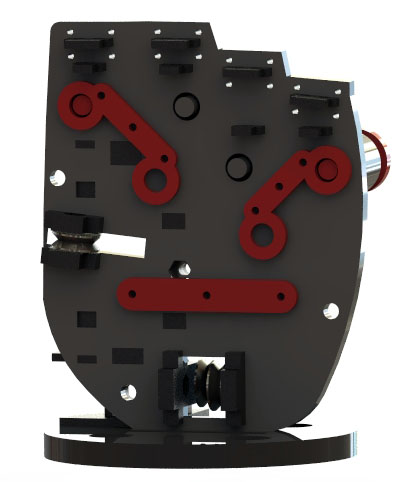
\includegraphics[width=8cm]{figures/paper_images/whiffletree.jpg}
\end{center}
\caption{Inner side of the palm. The three bars of the proposed whiffletree are depicted with red color. The holes of the upper two bars are filled by the elongated parts of the corresponding buttons, constraining the motion of different fingers. In this instance the motion of the index and pinky fingers is constrained, resulting to a change at the inclination of the differential mechanism finger bars.} 
\label{differential}
\end{figure}

\subsection{Fabrication Techniques and Personalized Design}

All files (CAD files, codes) required for the replication and control of the proposed robot hands, are available for download through the OpenBionics initiative \cite{Liarokapis2014ASURRW} website at the following URL:
\begin{center}{\small{\url{http://www.openbionics.org}}}\end{center} 

 The proposed design is essentially 2D and can be replicated with various fabrication techniques. In particular, we provide 3D models (.stl files) that can be used for fabrication with rapid prototyping techniques such as 3D printing and 2D models (.dwg, .dxf and other CAD files) that can be used for fabrication with laser cutting machines or other standard machining tools. The proposed hands are made out of off-the-shelf, low-cost materials. All required materials can be easily found in hardware stores around the world. 

 \begin{figure}[h]
\begin{center}
\begin{tabular}[50]{ c c }
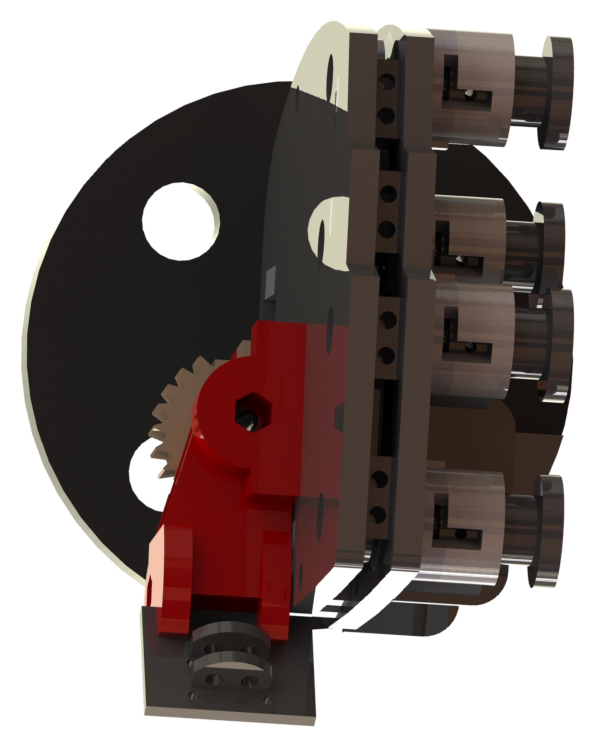
\includegraphics[height=9cm]{figures/paper_images/buttons.JPG}&
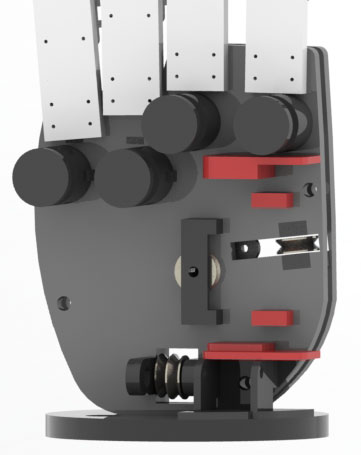
\includegraphics[height=9cm]{figures/paper_images/servobase.jpg}\\
{{a) thumb mechanism}} & {{b) servo base}}\\
\end{tabular}
\end{center}
\caption{Subfigure a) depicts the thumb mechanism in red and golden colors. Subfigure b) depicts the servo base of the HerkuleX servo motor in red. In both subfigures the buttons that implement the differential tree locking are denoted with black color.} 
\label{palm}
\end{figure} 

For reference, we provide the finger design parameters for a prosthetic hand with length 19 cm in Table \ref{fingerparameters}, while other complementary features are reported in Table \ref{handcharacteristics}. It should be pointed out that both the weight and the cost of the proposed hand design are significantly low, 300 g and $<$200 USD respectively. 

\begin{table}[ht!]
\caption{Finger characteristics for a robot hand with length 19cm} \label{fingerparameters}
\begin{center}
\begin{tabular}[50]{ c c c c c }
{\it{Finger}} & {\it{Weight}} & {\it{Length}} & {\it{Breadth}} & {\it{Width}}\\
\hline
{Index} & {30 g} & {88 mm} & {16.2 mm} & {15 mm}\\
{Middle} & {30 g} & {98 mm} & {16.2 mm} & {15 mm}\\
{Ring} & {30 g} & {95 mm} & {16.2 mm} & {15 mm}\\
{Pinky} & {25 g} & {76 mm} & {16.2 mm} & {15 mm}\\
{Thumb} & {20 g} & {68 mm} & {16.2 mm} & {15 mm}\\
\end{tabular}
\end{center}
\end{table} 

\begin{table}[ht!]
\caption{Hand characteristics} \label{handcharacteristics}
\begin{center}
\begin{tabular}[50]{ c c c c c }
{\it{Cost}} &  {\it{Weight}} & {\it{Length}} & {\it{Breadth}} & {\it{Width}}\\
$<$ 200 USD & 300 g & 190 mm & 90 mm & 62.50 mm 
\end{tabular}
\end{center}
\end{table} 

 \begin{figure}[ht]
\centering
\begin{tabular}[50]{ c c c c }
{\it{Front}} & {\it{Side 1}} & {\it{Side 2}} & {\it{Back}}\\
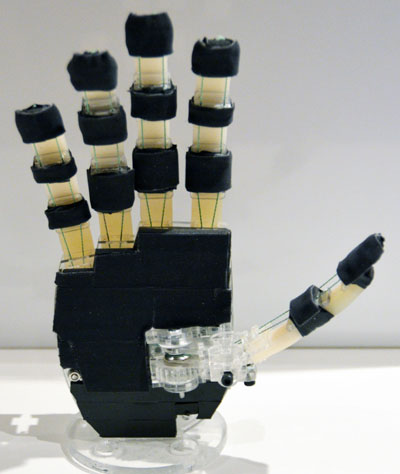
\includegraphics[height=3.4cm]{figures/paper_images/hand1.jpg}&
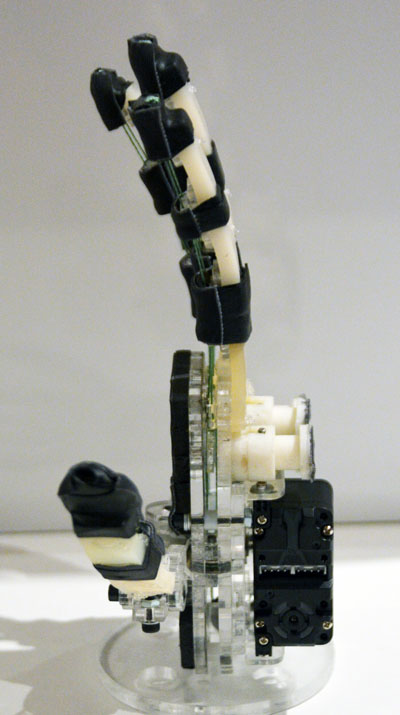
\includegraphics[height=3.4cm]{figures/paper_images/hand2.jpg}&
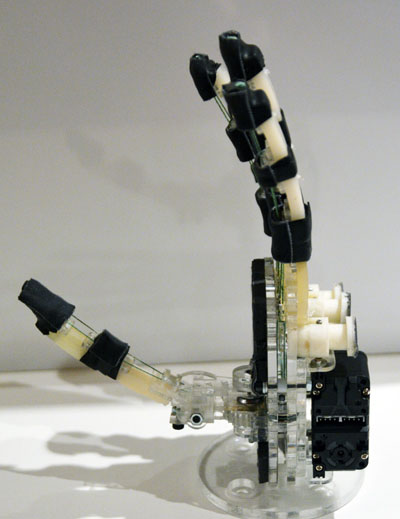
\includegraphics[height=3.4cm]{figures/paper_images/hand3.jpg}&
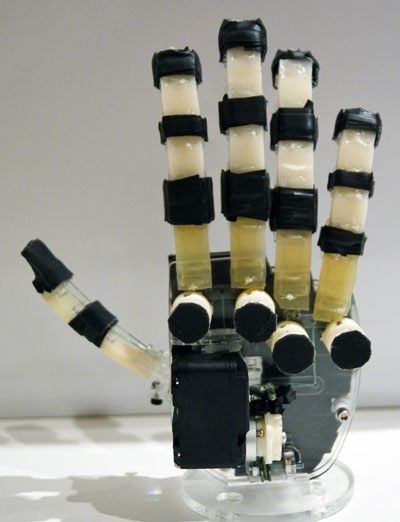
\includegraphics[height=3.4cm]{figures/paper_images/hand4.jpg}\\
\end{tabular}
\caption{Different views of the prosthetic hand developed.} 
\label{RobotHandViews}
\end{figure} 

\section{Results \& Experiments}

The performance capabilities of the proposed design have already been validated with extensive experimental paradigms that include: 1) grasping of a wide range of everyday life objects, 2) execution of a series of daily living tasks. For the experiments, we used an Arduino Micro platform \cite{Arduino} to control the HerkuleX DRS0201 servo motor, a custom made PCB module that connects the arduino platform with the servo motor and the ROS package (written in Python) that we created within the context of the OpenBionics initiative (available at \url{https://github.com/OpenBionics}). In the following sections we evaluate the performance of the proposed prosthetic hands.

\subsection{Force Exertion Capability}

Fig. \ref{forcedisplacement} contains diagrams demonstrating the relationships between the linear displacement of the tendon and the force applied at the fingertips, with and without finger blocking, for various hand postures. This can be useful for performing precision grasps, since blocking a subset of fingers leads to increased force transmission for the remaining free fingers.


\begin{figure}[h]
\centering
\begin{tabular}{ c c c }
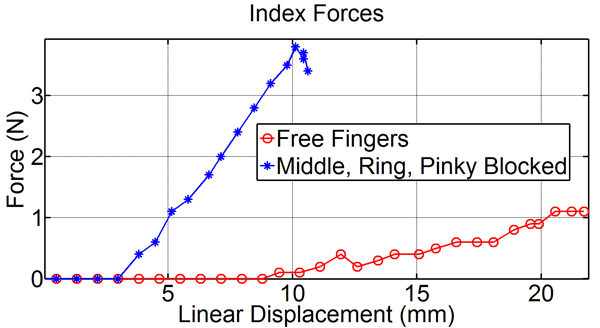
\includegraphics[scale=0.22]{figures/paper_images/indexforces.jpg} &
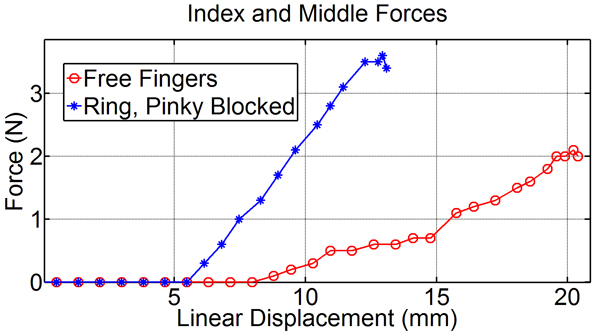
\includegraphics[scale=0.22]{figures/paper_images/indexmiddleforces.jpg} &
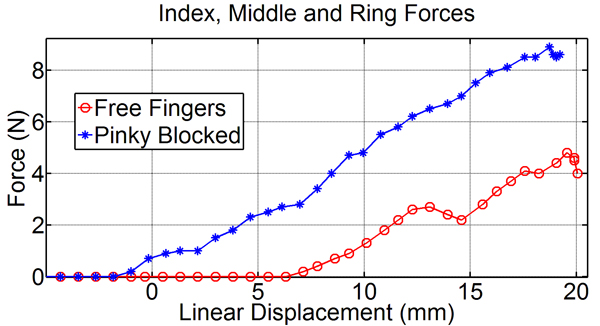
\includegraphics[scale=0.22]{figures/paper_images/indexmiddleringforces.jpg}\\ 
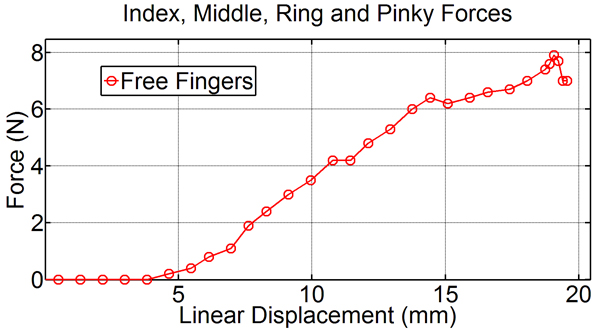
\includegraphics[scale=0.22]{figures/paper_images/fingersforces.jpg} & 
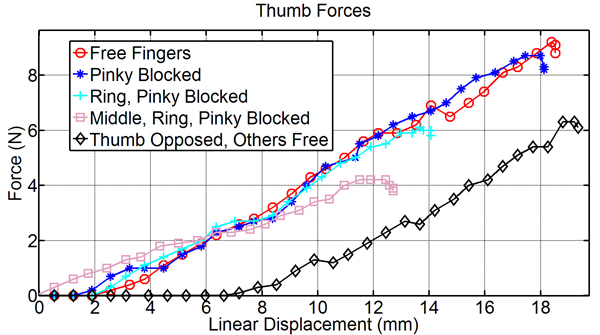
\includegraphics[scale=0.22]{figures/paper_images/thumbforces.jpg}
\end{tabular}
\caption{Relationship between tendon displacement and finger forces for various postures.} 
\label{forcedisplacement}
\end{figure}

\subsection{Implementing Various Grasping Postures and Common Gestures}

The efficacy of the selectively lockable differential mechanism was validated through a plethora of experiments.  The user was pressing the locking buttons to achieve different postures. This functionality is not only important for grasping (where the user is able to choose a preferred grasping strategy / posture), but also for: 1) implementing specific gestures (e.g., making the peace sign or showing a number), 2) reaching for an object located at a narrow space (task that might require less than five fingers), or 3) execute non-prehensile manipulation tasks (e.g., press a button or move a slider on a console). Figs. \ref{Locked} and \ref{Free} depict various postures, achieved by pressing different sets of buttons. 

\begin{figure}[ht]
\begin{center}
\scalebox{0.95}{
\begin{tabular}[50]{ c c c c }
{\it{Index}} & {\it{Middle}} & {\it{Ring}} & {\it{Pinky}}\\
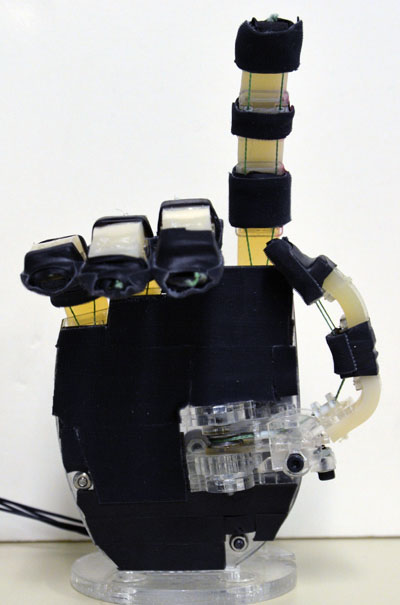
\includegraphics[height=5cm]{figures/paper_images/index.jpg}&
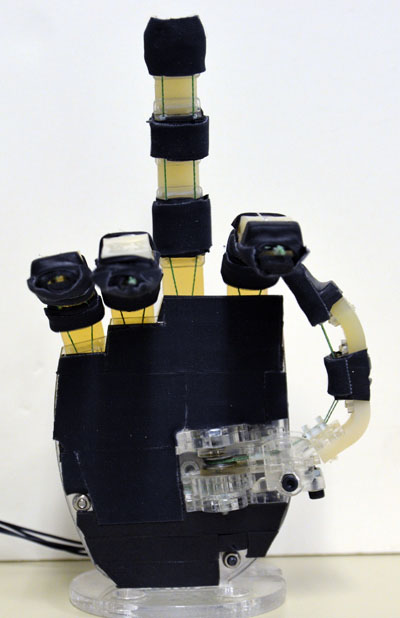
\includegraphics[height=5cm]{figures/paper_images/middle.jpg}& 
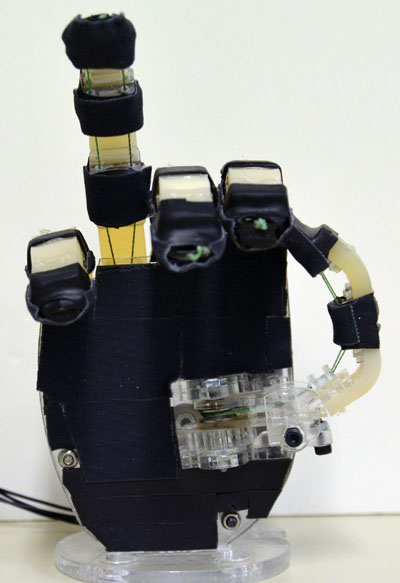
\includegraphics[height=5cm]{figures/paper_images/ring.jpg}&
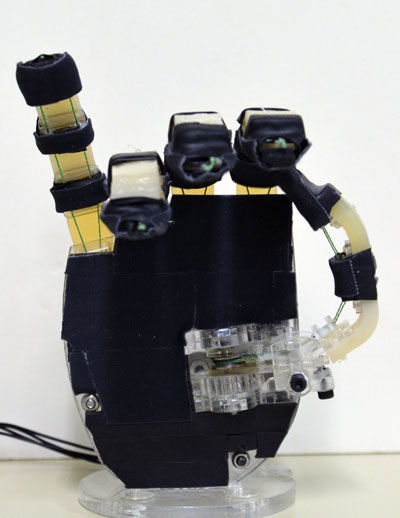
\includegraphics[height=5cm]{figures/paper_images/pinky.jpg}\\
\end{tabular}
}
\end{center}
\caption{Four different postures are depicted. All fingers except one are closing. The locked finger can be used to: 1) press buttons, 2) to reach something in narrow spaces, 3) to implement specific gestures or 4) to execute non-prehensile manipulation tasks (e.g., moving a slider).} 
\label{Locked}
\end{figure} 


\begin{figure}[ht]
\begin{center}
\begin{tabular}{ c c c c }
{\it{M, R, P}} & {\it{I, M}} & {\it{I, M, P}} & {\it{I, P}}\\
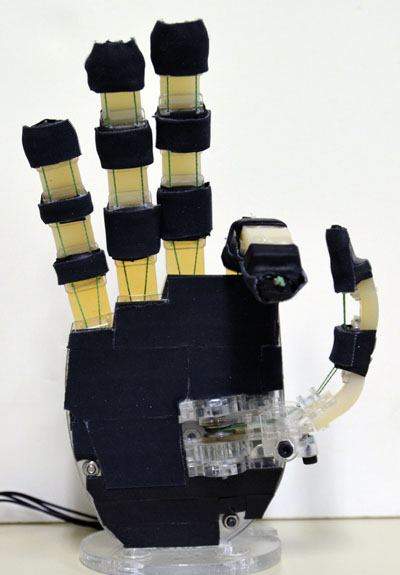
\includegraphics[height=5cm]{figures/paper_images/index_free.jpg}&
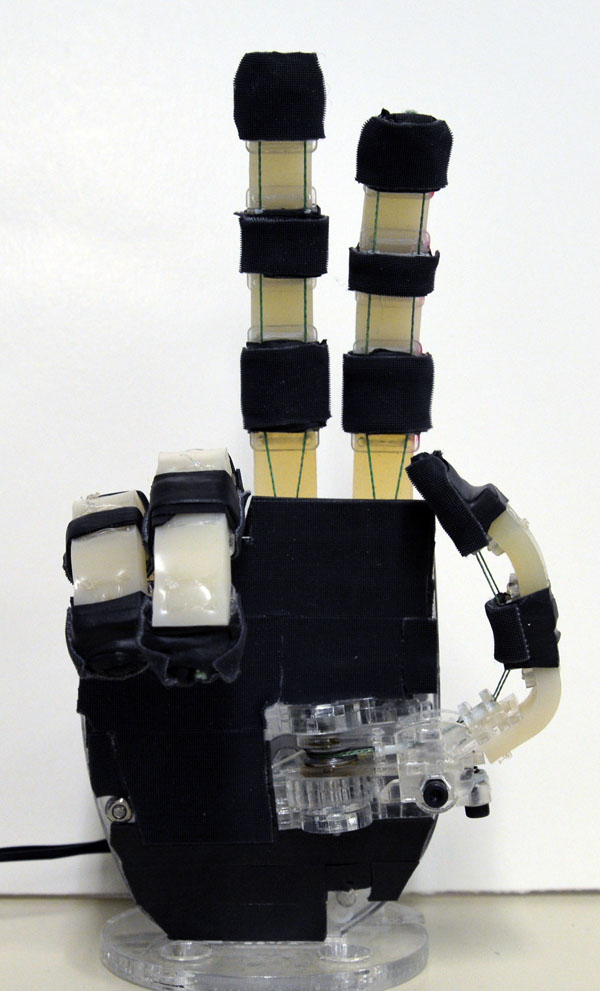
\includegraphics[height=5cm]{figures/paper_images/peace.jpg}& 
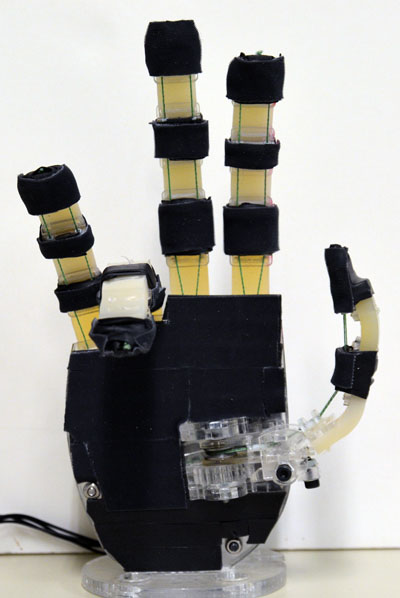
\includegraphics[height=5cm]{figures/paper_images/ring_free.jpg}&
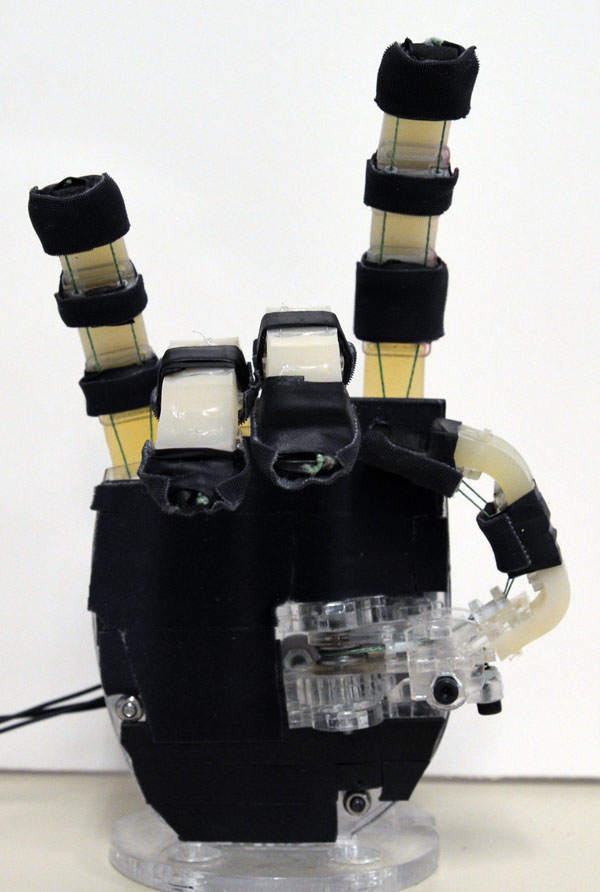
\includegraphics[height=5cm]{figures/paper_images/metal.jpg}\\
\end{tabular}
\end{center}
\caption{Four different postures are depicted. The differential mechanism allows for different grasping postures and hand gestures to be achieved. With the letters I, M, R and P we denote that motion of the index, middle, ring and pinky finger respectively, is constrained.} 
\label{Free}
\end{figure}

\subsection{Grasping Everyday Life Objects}

The actual grasping capabilities of the hand were tested through a set of experiments during which the user grasped a wide range of everyday life objects, to execute common daily living activities. For these experiments we used 1) a mug, 2) a soap, 3) a magazine, 4)  a marker, 5) a pair of glasses, 6) a large rectangular box, 7) a glass cleaner spray, 8) a 1.5L bottle of water, 9) a glass of water and 10) a spoon. Regarding the daily living tasks, the hand is used: 1) to serve water from a 1.5L bottle to a glass, 2) to stir the water inside the glass with a spoon and 3) to position a series of tools to their cases and put them inside a rectangular box. Instances of the conducted experiments are displayed in Fig. \ref{Experiments}. All experiments were recorded and the video can be found (in HD quality), at the following URL: 
\begin{center}{\small{\url{http://www.openbionics.org/videos/}}}\end{center}

More details about the experiments and the possible applications, can be found in \cite{Kontoudis2015IROS}, as well as at the official website of the OpenBionics initiative:

\begin{center}
{\url{http://www.openbionics.org}}
\end{center} 

\begin{figure}[ht!]
\centering
\scalebox{0.98}{
\begin{tabular}[50]{ c c c c }
{\it{Mug}} & {\it{Marker}} & {\it{Sunglasses}} & {\it{Bottle}}\\
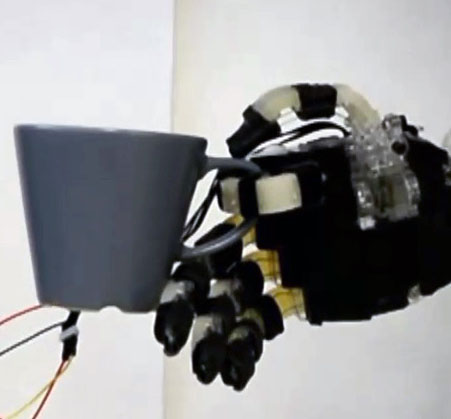
\includegraphics[height=4cm]{figures/paper_images/experiment1.jpg}&
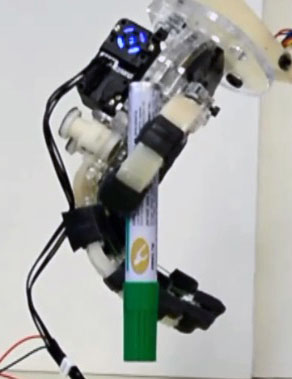
\includegraphics[height=4cm]{figures/paper_images/experiment2.jpg}&
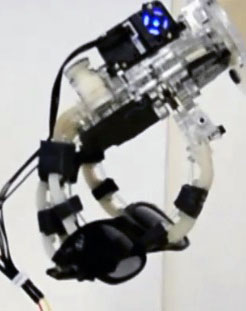
\includegraphics[height=4cm]{figures/paper_images/experiment3.jpg}&
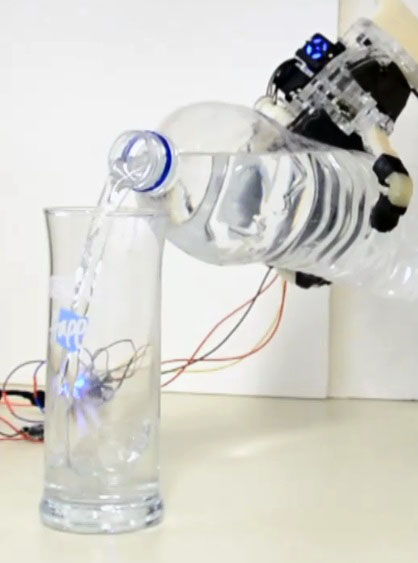
\includegraphics[height=4cm]{figures/paper_images/experiment4.jpg}\\
\end{tabular}
}
\caption{Images from the experiments conducted. Five different everyday life objects are grasped in order to execute different tasks: 1) a coffee mug is grasped from the handle in order to drink from it, 2) a marker is grasped in order to write, 3) a pair of glasses are picked up and 4) a 1.5L bottle is grasped in order to serve water.} 
\label{Experiments}
\end{figure} 

\newpage


%%%% Appendices %%%% 

\section{Necessary Tools and Materials}

Our prosthetic hand can be assembled using the following tools and materials that can be easily found in hardware stores around the world.

\begin{center}
\begin{tikzpicture}
\node [mybox] (box){
	\scalebox{1.07}{
	\begin{tabular}{ c c }
		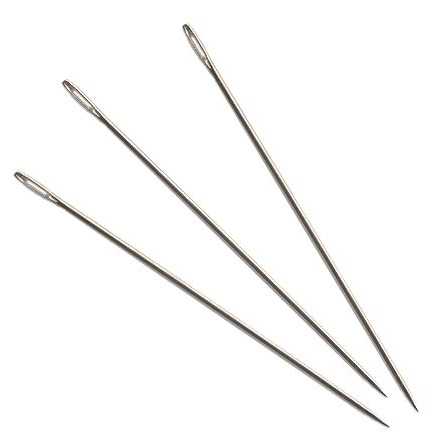
\includegraphics[width=2cm]{figures/Tools/needles.jpg} &
		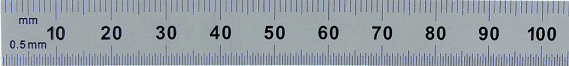
\includegraphics[width=5cm]{figures/Tools/ruler.png} 
		\\
		Long Needles [D:1mm, L:70mm] & Precision Ruler
		\\
		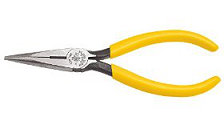
\includegraphics[width=3cm]{figures/Tools/NeedleNosePliers.png} &
		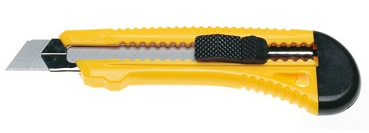
\includegraphics[width=4cm]{figures/Tools/Cutter.jpg} 
		\\
		 Long-Nose Pliers with Side-Cutting & Cutter
		\\
		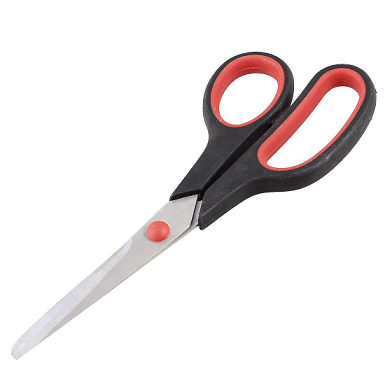
\includegraphics[width=3cm]{figures/Tools/scissors.png} &
		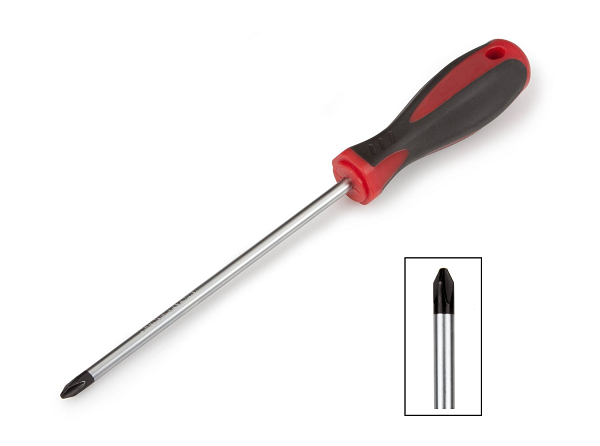
\includegraphics[width=4cm]{figures/Tools/ScrewDriver.png}
		\\
		Scissors & Phillips Screwdriver [no. 1,2]
		\\
		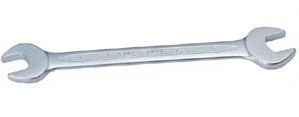
\includegraphics[width=3cm]{figures/Tools/Open-endWrench.jpg} &
		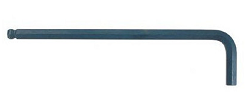
\includegraphics[width=4cm]{figures/Tools/AllenWrench.png}
		\\
		Open-End Wrench [M3 Hex Nut] & Allen Wrench [2.5mm]		
		\\
    	\end{tabular}
}
};
\node[mytitle, right=10pt] at (box.north west) {Board 4.1: Tools};
\end{tikzpicture}%
\end{center}

\begin{center}
\begin{tikzpicture}
\node [mybox] (box){
	\scalebox{.98}{
	\begin{tabular}{ c c c }
		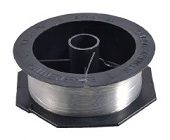
\includegraphics[width=2.0cm]{figures/Tools/FishingLine.jpg} &
                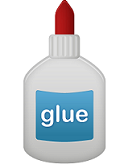
\includegraphics[width=1.5cm]{figures/Tools/Glue.jpg} &
                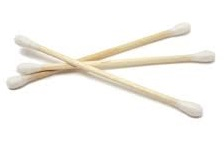
\includegraphics[width=2.5cm]{figures/Tools/Swabs.jpg}\\
		Dyneema Fishing Line [0.4mm] & ABS Glue & Ear Cotton Swabs\\
		\& Nylon Fishing Line [0.4mm] & & \\
		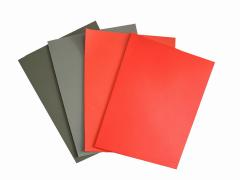
\includegraphics[width=2.5cm]{figures/Tools/Silicone.jpg} &
                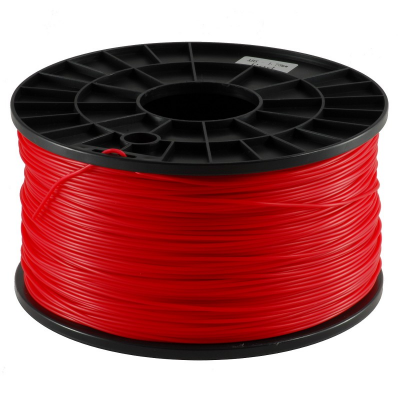
\includegraphics[width=2.0cm]{figures/Tools/ABS_3mm.jpg} & 
                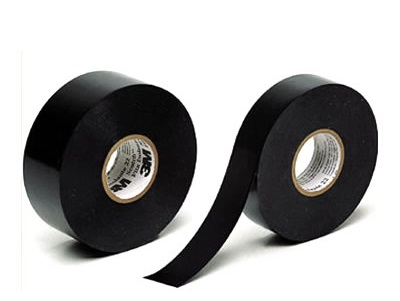
\includegraphics[width=2.5cm]{figures/Tools/Tapes.jpg}
                \\
		Silicone Sheets [4mm, 5mm] & ABS filament [3mm] & Sponge, Self-Adhesive \\
		& & \& Anti-Slip Tapes \\
    	\end{tabular}
	}
};
\node[mytitle, right=10pt] at (box.north west) {Board 4.2:  Materials};
\end{tikzpicture}%
\end{center}

\section{Parts Reference}

In this section we list all the necessary parts for the assembly of the prosthetic hand. The parts are divided in three categories: i) the finger parts, ii) the palm parts and iii) the auxiliary parts. The first category consists of all required parts to build all 5 hand fingers, the second category consists of the main palm parts, i.e., the palm structure and the whiffletree mechanism while the third category contains all required parts for building the Herkulex DRS201 servo base, the thumb mechanism, the tendon routing system and the buttons. 


In the following sections we provide a table for each category, listing all parts, along with the names of their corresponding Solidworks part files, their quantity and usage as well as an indication of whether they can be 3D printed. We also provide a separate table with all parts that can be 3D printed. Finally, to facilitate the identification of each part, we provide images of the models. 

\subsection{Finger Parts}



\begin{table}[h!]
	\centering
	\scalebox{0.87}{
		\begin{tabular}{ | l | l | l |}
			\hline
			\multicolumn{3}{|c|}{\bf{Finger Parts List}} \\
			\hline
			{\bf{Part Name}} & {\bf{Qty}} & {\bf{Description}}\\ \hline
			index & 1 & Index Finger [3D printer] \\ \hline
			middle & 1 & Middle Finger [3D printer] \\ \hline
			ring & 1 & Ring Finger [3D printer] \\ \hline
			pinky & 1 & Pinky Finger [3D printer] \\ \hline
			thumb & 1 & Thumb Finger [3D printer] \\ \hline    	
			tubePIP & 10 & Cotton Swab Tube for PIP [d:2mm, D:2.5mm, L:depending on the finger]  \\ \hline
			tubeMIP & 10 & Cotton Swab Tube for MIP [d:2mm, D:2.5mm, L:depending on the finger]  \\ \hline
			tubeDIP & 10 & Cotton Swab Tube for DIP [d:2mm, D:2.5mm, L:depending on the finger]  \\ \hline
			Joint DIP \& MIP & 5 & Silicone Sheet, 60A Durometer  [(Joint Lengthx16.2x4)mm]\\ \hline
			Joint PIP & 5 & Silicone Sheet, 60A Durometer [(Joint Lengthx16.2x5)mm]\\ \hline
			Dyneema Fishing Line & 1 & Tendon Routing [D:0.4mm, Strength:41.5kg] \\ \hline
			Deformable Spong-like Tape & 1 & [Width:10mm, Thickness:5mm] \\ \hline
			Anti-Slip Tape & 1 & 3M Gripping Material [Width:25mm] \\ \hline
			Self-Adhesive Tape & 1 & 3M Scotch 23 [Width:20mm] \\ \hline
		\end{tabular}
	}
\end{table}

\begin{center}
	\begin{tikzpicture}
	\node [mybox] (box){%
		\begin{tabular}{ c c c c}
		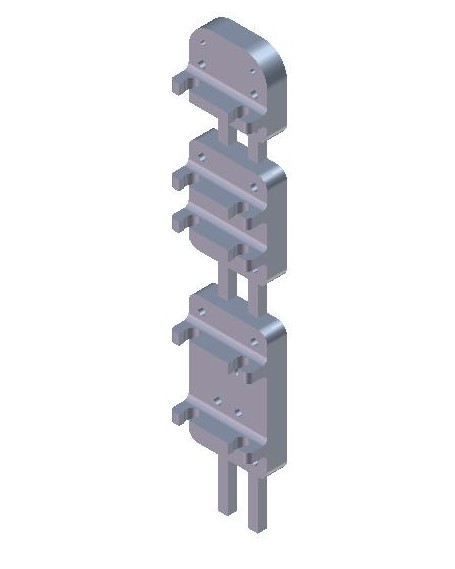
\includegraphics[width=2.8cm]{figures/Parts/index.jpg}   &
		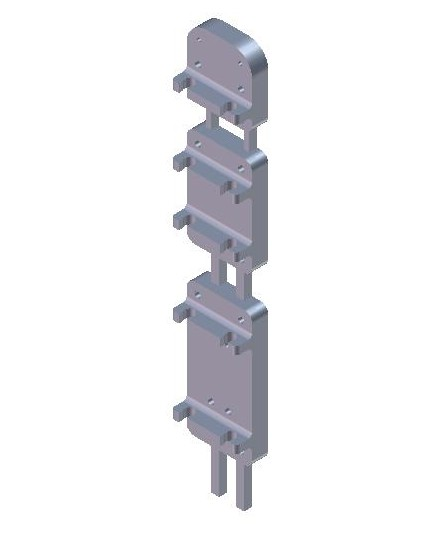
\includegraphics[width=3.0cm]{figures/Parts/middle.jpg}  &
		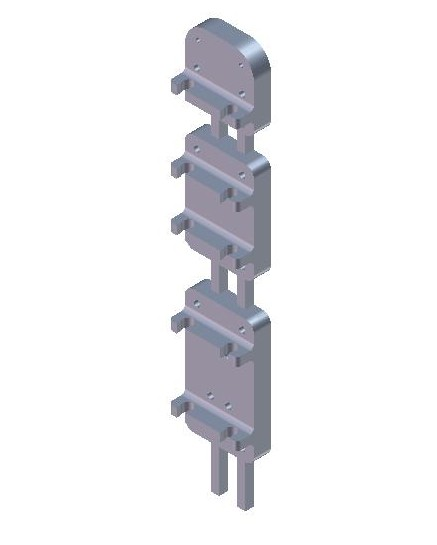
\includegraphics[width=3.0cm]{figures/Parts/ring.jpg}	&
		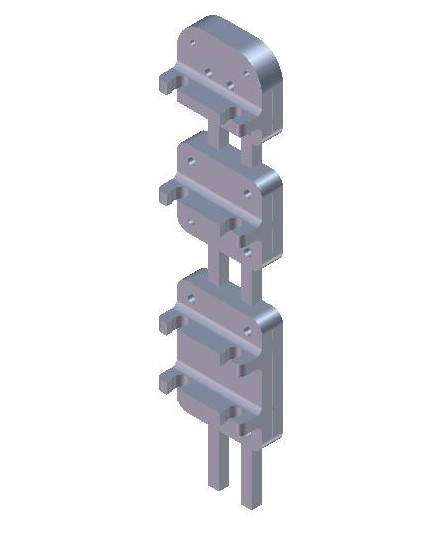
\includegraphics[width=2.7cm]{figures/Parts/pinky.jpg}	\\
		Index &  Middle & Ring & Pinky \\ \\
		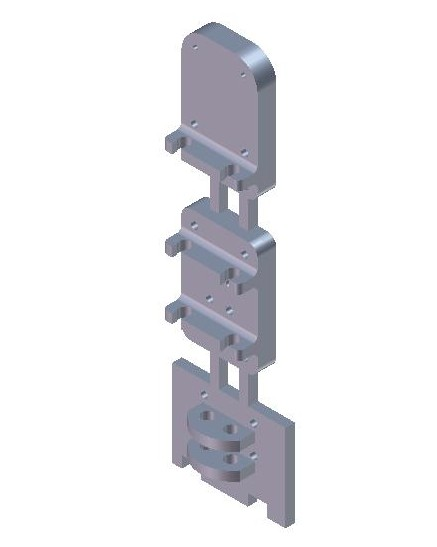
\includegraphics[width=2.7cm]{figures/Parts/thumb.jpg} &
		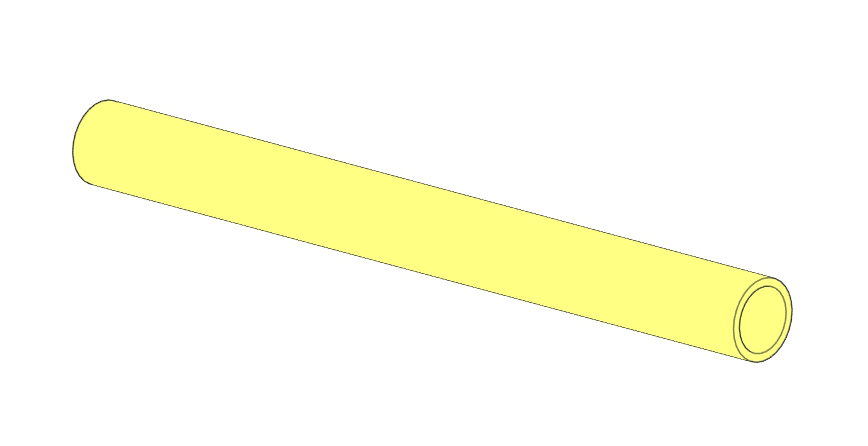
\includegraphics[width=3.0cm]{figures/Parts/Tube.png} &
		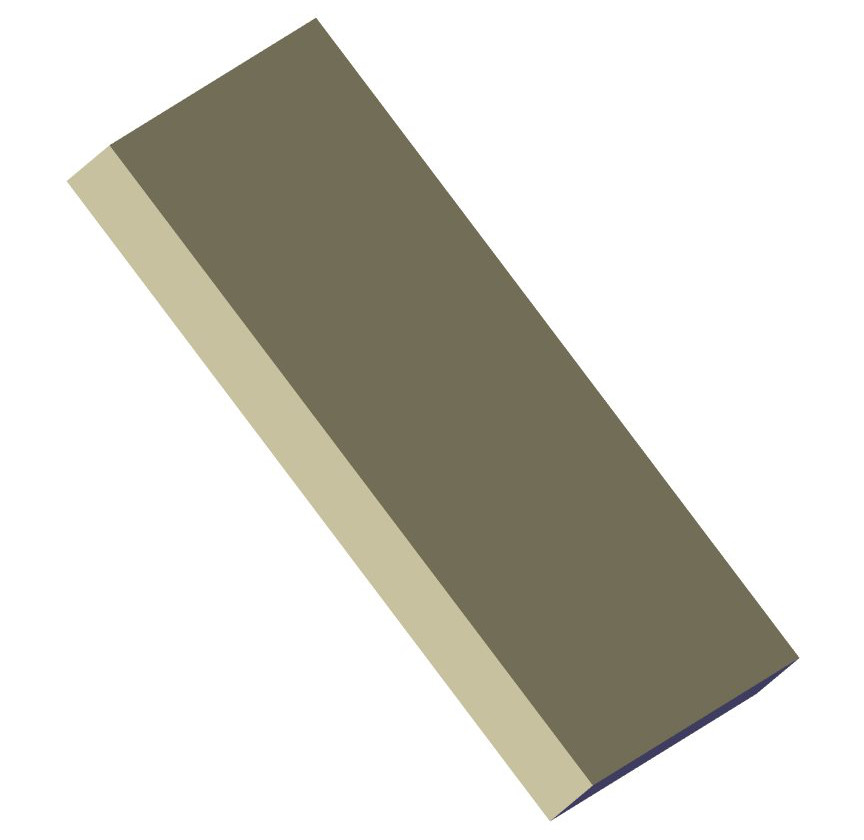
\includegraphics[width=3.0cm]{figures/Parts/SiliconeSheet.jpg} \\
		Thumb & tubes & Joint1, Joint2  \\ \\
		%		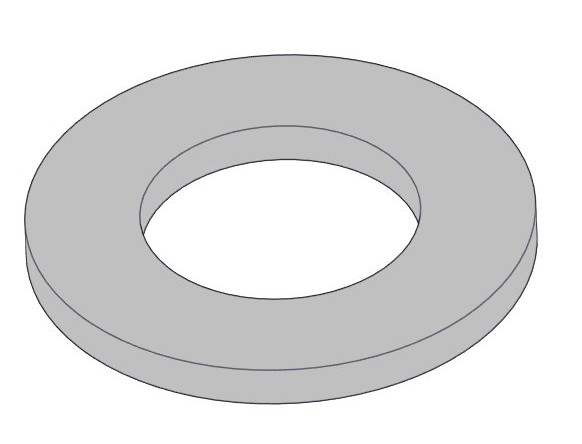
\includegraphics[width=0.9cm]{figures/Parts/WasherM3.jpg} &
		%		\includegraphics[width=1.8cm]{figures/Parts/ScrewM3x12.jpg} \\		
		%		\includegraphics[width=1cm]{figures/Parts/NutM3.jpg} &
		%		\includegraphics[width=1.4cm]{figures/Parts/Pulley.jpg} \\
		%		M3Nut & pulley  
		\end{tabular}
	};
	\node[mytitle, right=10pt] at (box.north west) {Board 5.1.1: Finger Parts};
	\end{tikzpicture}%
\end{center}

\newpage

\subsection{Palm Parts}


\begin{table}[h!]
	\centering
	\scalebox{0.84}{
		\begin{tabular}{ | l | l | l |}
			\hline
			\multicolumn{3}{|c|}{{\bf{Palm Parts List}}} \\
			\hline
			{\bf{Part Name}} & {\bf{Qty}} & {\bf{Description}}\\ \hline
			palmUp & 1 & Upside of Palm [3D printer] \\ \hline
			PalmDown & 1 & Downside of palm [3D printer] \\ \hline
			barIndexMiddle & 1 & Index \& Middle Fingers Whiphlee Tree Bar [3D printer] \\ \hline
			barRingPinky & 1 & Ring \& Pinky Fingers Whiphlee Tree Bar [3D printer] \\ \hline
			mainBar & 1 & 4 Fingers Whiphlee Tree Bar [3D printer] \\ \hline
			basePulleyInsidePalm & 4 & Tendon Routing of Thumb \& Mount of Base Flange [3D printer] \\ \hline   	    	    	    	
			Dyneema Fishing Line & 1 & Tendon Routing [D:0.4mm, Strength:41.5kg] \\ \hline
			Rubber Foam Tape & 1 & Tape for Palm [Width:10mm, Thickness:4mm] \\ \hline
			Anti-Slip Tape & 1 & 3M Gripping Material [Width:25mm] \\ \hline
			pulley & 1 & V-Groove Sealed Ball Bearing [d:3mm, D:12mm, B:4mm, Deepness:1.2mm] \\ \hline
			PlasticSpacer & 2 & Fastener [d:3.1mm, D:6mm, L:4mm] \\ \hline
			M3X12 Set Screw & 1 & Fastener, M3 Set Screw [L:12mm] \\ \hline	
			M3x16 Socket Cup Screw & 1 & Fastener, M3 Socket Cup Screw [L:16mm] \\ \hline
			M3x20 Socket Cup Screw & 2 & Fastener, M3 Socket Cup Screw [L:20mm] \\ \hline
			M3 Washer & 5 & Fastener, M3 [D:7.5, L:0.5mm] \\ \hline
			M3 Nut & 5 & Fastener, M3 Hex Nut \\ \hline
		\end{tabular}
	}
\end{table}

\vspace{0.2cm}

\begin{center}
	\begin{tikzpicture}
	\node [mybox] (box){%
		\scalebox{0.95}{
		\begin{tabular}{ c c c c }
		\includegraphics[width=3.5cm]{figures/Parts/palmUp.jpg} &
		\includegraphics[width=3.2cm]{figures/Parts/barIndexMiddle.jpg} &
		\includegraphics[width=3cm]{figures/Parts/barRingPinky.jpg} & 
		\includegraphics[width=1cm]{figures/Parts/PlasticSpacer.jpg} \\
		palmUp & barIndexMiddle & barRingPinky & PlasticSpacer \\
		\includegraphics[width=3.3cm]{figures/Parts/palmDown.jpg} &
		\includegraphics[width=4cm]{figures/Parts/mainBar.jpg} &
		\includegraphics[width=2cm]{figures/Parts/basePulleyInsidePalm.jpg} &
		\includegraphics[width=0.9cm]{figures/Parts/M3ThreadRod.jpg} \\
		palmDown & mainBar & basePulleyInsidePalm & M3X12 Set Screw \\
		\includegraphics[width=1.4cm]{figures/Parts/Pulley.jpg} &
		\includegraphics[width=1.8cm]{figures/Parts/ScrewM3x12.jpg} &
		\includegraphics[width=0.9cm]{figures/Parts/WasherM3.jpg} &
		\includegraphics[width=1.4cm]{figures/Parts/NutM3.jpg} \\
		pulley & M3x16, M3x20 & M3 Washer & M3 Nut  \\
		 & Socket Cup Screw & & \\ \\
		\end{tabular}
		}
	};
	\node[mytitle, right=10pt] at (box.north west) {Board 5.2.1: Palm Parts};
	\end{tikzpicture}%
\end{center}

\newpage

\subsection{Auxiliary Parts}

\begin{table}[h!]
	\centering
	\scalebox{0.8}{
		\begin{tabular}{ | l | l | l |}
			\hline
			\multicolumn{3}{|c|}{{\bf{Auxialiary Parts List}}} \\
			\hline
			{\bf{Part Name}} & {\bf{Qty}} & {\bf{Description}}\\ \hline
			baseHerkulex & 1 & Base of HerkuleX DRS201 [3D printer] \\ \hline
			toothedMechanism & 1 & Toothed Mechanism of Base Thumb [3D printer] \\ \hline
			toothedBlockMechanism & 1 & Toothed Block Mechanism of Thumb [3D printer] \\ \hline
			thumbMovingMechanism & 1 & Thumb Moving Mechanism [3D printer] \\ \hline
			thumbButton & 1 & Thumb Base Button [3D printer] \\ \hline
			lockMechanismSupport & 1 & Support of Thumb Lock Mechanism [3D printer] \\ \hline
			lockMechanismBracket & 2 & Bracket of Thumb Lock Mechanism [3D printer] \\ \hline
			pulleyServo & 1 & Pulley of Herkulex DRS201 [3D printer] \\ \hline
			supportPulley1 & 2 & Support pulleys of tendon routing system [3D printer] \\ \hline
			supportPulleyPalmUpAssem & 1 & Support pulley of tendon routing system [3D printer] \\ \hline  	
			dovetailFemale & 1 & Dovetail Female Flange [3D printer] \\ \hline
			flangePlate & 1 & Standard Flange Plate [3D printer] \\ \hline
			buttonBase & 4 & Base of Button [3D printer] \\ \hline    	
			buttonFrame & 4 & Frame of Button [3D printer] \\ \hline 
			buttonAxle & 4 & Axle of Button [3D printer] \\ \hline     	    	    	
			Dyneema & 1 & Tendon Routing [D:0.4mm, Strength:41.5kg] \\ \hline
			HerkulexDRS-201 & 1 & Actuator\\ \hline
			pulley & 4 & V-Groove Sealed Ball Bearing [d:3mm, D:12mm, B:4mm, Deepness:1.2mm] \\ \hline
			
			PlasticSpacer & 4 & Fastener [d:3.1mm, D:6mm, L:4mm] \\ \hline
			M3X18 Set Screw & 3 & Fastener, M3 Set Screw [L:18mm]  \\ \hline	
			M3X30 Set Screw & 1 & Fastener, M3 Set Screw [L:30mm]  \\ \hline	
			M3x6 Socket Cup Screw & 1 & Fastener, M3 Socket Cup Screw [L:6mm] \\ \hline
			M3x10 Socket Cup Screw & 1 & Fastener, M3 Socket Cup Screw [L:10mm] \\ \hline
			M3 Nut & 10 & Fastener, M3 Hex Nut \\ \hline
			M3 Washer & 4 & Fastener, M3 [D:7.5mm, L:0.5mm] \\ \hline
			M2x10 Machine Screw & 4 & Fastener, M2 Machine Screw [L:10mm] \\ \hline
			M2 Nut & 4 & Fastener, M2 Hex Nut \\ \hline
			M2x16 Dowel Pin & 4 & M2 Dowel Pin [L:16mm] \\ \hline
			Compression Spring 6mm L, 9mm OD, 1mm WD & 4 & 9mm Outer Dimension, 1mm Wire Diameter [L:6mm]\\ \hline
		    Compression Spring 3mm L, 3.5mm OD, 0.5mm WD & 1 & 3.5mm Outer Dimension, 0.5mm Wire Diameter [L:3mm]  \\ \hline
		\end{tabular}
	}
\end{table}

\vspace{0.2cm}

\begin{center}
	\begin{tikzpicture}
	\node [mybox] (box){%
		\begin{tabular}{ c c c }
		\includegraphics[width=3.1cm]{figures/Parts/baseHerkulex.jpg} &
		\includegraphics[width=2.7cm]{figures/Parts/thumbMovingMechanism.jpg} &
		\includegraphics[width=3.3cm]{figures/Parts/pulleyServo.jpg} \\
		baseHerkulex & thumbMovingMechanism & pulleyServo \\
		\includegraphics[width=3.4cm]{figures/Parts/toothedMechanism.jpg} &
		\includegraphics[width=1.9cm]{figures/Parts/thumbButton.jpg} & 
		\includegraphics[width=2.2cm]{figures/Parts/toothedBlockMechanism.jpg} \\
		 toothedMechanism & thumbButton & toothedBlockMechanism  \\
		\includegraphics[width=2.3cm]{figures/Parts/lockMechanismBracket.jpg} &
		\includegraphics[width=1.6cm]{figures/Parts/lockMechanismSupport.jpg} \\
		 lockMechanismBracket &  lockMechanismSupport \\
		
		\end{tabular}
	};
	\node[mytitle, right=10pt] at (box.north west) {Board 5.3.1: Auxiliary Parts I};
	\end{tikzpicture}%
\end{center}

\newpage

\begin{center}
	\begin{tikzpicture}
	\node [mybox] (box){%
		\scalebox{0.92}{
		\begin{tabular}{ c c c }
		\includegraphics[width=2.7cm]{figures/Parts/supportPulley1.jpg} &
		\includegraphics[width=2.7cm]{figures/Parts/supportPulleyPalmUpAssem.jpg} & 
		\includegraphics[width=3cm]{figures/Parts/dovetailFemale.jpg} \\
		supportPulley1 & supportPulleyPalmUpAssem & dovetailFemale \\ \\
		\includegraphics[width=5cm]{figures/Parts/FlangePlate.jpg} &
		\includegraphics[width=2.1cm]{figures/Parts/buttonBase.jpg} &
		\includegraphics[width=2.1cm]{figures/Parts/buttonFrame.jpg} \\
		flangePlate & buttonBase & buttonFrame \\ \\
		\includegraphics[width=3cm]{figures/Parts/buttonAxle.jpg} &		
		\includegraphics[width=1.4cm]{figures/Parts/Pulley.jpg} &
		\includegraphics[width=1cm]{figures/Parts/PlasticSpacer.jpg} \\
		buttonAxle & pulley & PlasticSpacer \\ \\
		\includegraphics[width=1.8cm]{figures/Parts/ScrewM3x12.jpg} &
		\includegraphics[width=1.4cm]{figures/Parts/NutM3.jpg} &
		\includegraphics[width=0.9cm]{figures/Parts/M3ThreadRod.jpg} \\
		M3x6, M3x10 & M3 Nut & M3X18, M3X30 \\ 
		Socket Cup Screw & & Set Screw \\ \\
		\includegraphics[width=0.9cm]{figures/Parts/WasherM3.jpg} & 
		\includegraphics[width=1.2cm]{figures/Parts/NutM3.jpg} &
		\includegraphics[width=1.6cm]{figures/Parts/ScrewM3x12.jpg} \\
		M3 Washer & M2 Nut & M2x10 Machine Screw \\ \\
		\end{tabular}
		}
	};
	\node[mytitle, right=10pt] at (box.north west) {Board 5.3.2: Auxiliary Parts II};
	\end{tikzpicture}%
\end{center}

\newpage

\subsection{3D Printed Parts}

The following table contains all parts that can be 3D printed. The corresponding STL files contained in the Prosthetic-Hands/CAD directory of our GitHub reporitory (\url{www.github.com/openbionics}) are appropriate to be used with a 3D printer. 


\vspace{0.2cm}

\begin{table}[h!]
	\centering
	\scalebox{0.8}{
		\begin{tabular}{ | l | l | l | l | }
			\hline
			\multicolumn{4}{|c|}{{\bf{3D Printer Parts}}} \\
			\hline
			{\bf{Part Name}} & {\bf{Qty}} & {\bf{Description}} & {\bf{TAZ ABS Profile}}\\ \hline
			index & 1 & Index Finger & Medium, Support Off  \\ \hline
			middle & 1 & Middle Finger & Medium, Support Off \\ \hline
			ring & 1 & Ring Finger & Medium, Support Off \\ \hline
			pinky & 1 & Pinky Finger & Medium, Support Off \\ \hline
			thumb & 1 & Thumb Finger & Medium, Support Off \\ \hline 
			palmUp & 1 & Upside of Palm & Medium, Support On \\ \hline
			PalmDown & 1 & Downside of palm & Medium, Support On \\ \hline
			barIndexMiddle & 1 & Index \& Middle Fingers Whiphlee Tree Bar & Medium, Support Off \\ \hline
			barRingPinky & 1 & Ring \& Pinky Fingers Whiphlee Tree Bar & Medium, Support Off \\ \hline
			mainBar & 1 & 4 Fingers Whiphlee Tree Bar & Medium, Support Off \\ \hline
			basePulleyInsidePalm & 4  & Tendon Routing of Thumb \& Mount of Base Flange & Medium, Support Off \\ \hline
			baseHerkulex & 1 & Base of HerkuleX DRS201 & Medium, Support On \\ \hline
			toothedMechanism & 1 & Toothed Mechanism of Base Thumb & Medium, Support Off \\ \hline
			toothedBlockMechanism & 1 & Toothed Block Mechanism of Thumb & Medium, Support Off \\ \hline
			thumbMovingMechanism & 1 & Thumb Moving Mechanism & Medium, Support On \\ \hline
			thumbButton & 1 & Thumb Base Button & Medium, Support Off \\ \hline
			lockMechanismSupport & 1 & Support of Thumb Lock Mechanism & Medium, Support Off \\ \hline
			lockMechanismBracket & 2 & Bracket of Thumb Lock Mechanism & Medium, Support Off \\ \hline
			pulleyServo & 1 & Pulley of Herkulex DRS201 & Medium, Support On \\ \hline
			supportPulley1 & 2 & Support pulleys of tendon routing system & Medium, Support Off \\ \hline
			supportPulleyPalmUpAssem & 1 & Support pulley of tendon routing system & Medium, Support On \\ \hline  	
			dovetailFemale & 1 & Dovetail Female Flange & Medium, Support On \\ \hline
			flangePlate & 1 & Standard Flange Plate & Medium, Support On \\ \hline
			buttonBase & 4 & Base of Button & Medium, Support On \\ \hline    	
			buttonFrame & 4 & Frame of Button & Medium, Support On \\ \hline 
			buttonAxle & 4 & Axle of Button & Medium, Support On \\ \hline
		\end{tabular}
	}
\end{table}

\vspace{1cm}

For the replication of the prosthetic hand we use the \href{https://download.lulzbot.com/TAZ/4.0/documentation/2014Q2/manual/TAZ_4_Manual.pdf}{LulzBot TAZ 4 3D Printer} and ABS material. We used the settings of the default TAZ Slic3r profiles which can be found \href{https://www.lulzbot.com/support/taz-slic3r-profiles}{here}, except from a small set of parameters that can be found on the following table.

\vspace{1cm}

\begin{table}[h!]
	\centering
	\scalebox{1}{
		\begin{tabular}{ | l | l |}
			\hline
			\multicolumn{2}{|c|}{{\bf{3D Printer Settings}}} \\ \hline
			{\bf{Parameter}} & {\bf{Value}} \\ \hline
			Infill, Fill Density & 20\% \\ \hline
			Infill, Fill Pattern & Honeycomb \\ \hline
			Seam Position & Random \\ \hline
			Brim, Brim Width & 2 mm \\ \hline
		\end{tabular}
	}
\end{table}

\newpage

\subsection{Before Assembling}

Before starting the assembly, the following steps should be followed: \\  \\
$\bullet$ Smoothen the acrylic parts with sandpaper. \\ \\
$\bullet$ Treat the ABS parts with acetone (e.g. see \href{http://blog.reprap.org/2013/02/vapor-treating-abs-rp-parts.html}{reprap Blog}).\\ \\
$\bullet$ Cut the cotton swabs to the appropriate size (following the parts reference dimensions). \\ \\
$\bullet$ Cut the silicone sheets to the appropriate size (following the parts reference dimensions). \\ \\
$\bullet$ Group the parts according to the parts reference. \\ \\
$\bullet$ Pay increased attention to the steps followed by the following icon: \circled{!}\\ \\
%$\bullet$ Note that the provided models do not have the actual size of the parts.\\ \\

\begin{center}
	\begin{tikzpicture}
	\node [mybox] (box){%
		\begin{tabular}{ c }
		\includegraphics[width=12cm]{figures/Parts/SilliconeCut.jpg} \\
		Cutting the silicone sheets with a cutter and a ruler.
		\end{tabular}
	};
	\node[mytitle, right=10pt] at (box.north west) {Board 5.5.1: Silicone Sheets Preparation};
	\end{tikzpicture}%

\end{center}


\section{Fingers Assembly}

This section contains instructions for assembling all 5 fingers of the prosthetic hand. Before each assembly step, a table containing all required materials and tools will be provided for convenience.

\subsection{Assembling the Phalanges}

%The parts and the materials you will need to assemble the fingers are listed in table \ref{phalangespartsmaterials}. The phalanges for all fingers of the hand can be assembled by gluing the parts of the following table, following the illustrated instructions of the the figures below. 

\begin{table}[ht!]
	\centering
	%\begin{minipage}[b]{0.50\linewidth}\centering
		\scalebox{1}{
			\begin{tabular}{ | c | c |}
				\hline
				\multicolumn{2}{|c|}{\bf{Part List 6.1.1}} \\
				\hline
				{\bf{Part Name}} & {\bf{Qty}}\\ \hline
				index & 1  \\ \hline
				middle & 1  \\ \hline
				ring & 1  \\ \hline
				pinky & 1  \\ \hline
				thumb & 1 \\ \hline
				tubeMIP & 8  \\ \hline
				tubePIP & 10  \\ \hline
				tubeDIP & 10  \\ \hline
				%		M3Washer & 16 \\ \hline
				%		M3Nut & 4 \\ \hline
				%		pulley & 4 \\ \hline
				\multicolumn{2}{|c|}{\textbf{Materials}} \\
				\hline
				\multicolumn{2}{|c|}{Super Glue } \\				
				\hline
			\end{tabular}				
		}
	%\end{minipage}
	
	%\caption{Parts and materials needed to assemble the phalanges.}
	%\label{phalangespartsmaterials}
\end{table}

%\begin{table}[ht!]
%	\centering
%	%\begin{minipage}[b]{0.50\linewidth}\centering
%
%	%\end{minipage}
%\end{table}



\begin{figure}[h]
	\centering
	\begin{tikzpicture}
	\node [mybox] (box){%
		\begin{minipage}[b]{0.45\textwidth}%\centering
		\begin{tabular}{ l l}
		{\circled{1}} & {Insert the low friction tubes to}\\
		{} & {the tubePIP/tubeMIP plates.} \\ \\
		{\circled{2}} & {Glue the edges of the tubes to}\\
		{} &  {the tube plates with super glue.}\\
		\end{tabular}
		\end{minipage}
		%\hspace{0.5cm}	
		\begin{minipage}[b]{0.4\textwidth}
		\begin{tabular}{ l }
		\includegraphics[width=6cm]{figures/Finger/Finger8.jpg}
		\end{tabular}
		\end{minipage}
	};
	%\node[anchor=south] at (-5,3.7) {\textbf{PIP and MIP Phalanges}}; % or (current bounding box.north) {Some Text};
	\node[mytitle, right=10pt] at (box.north west) {Board 6.1.1: Assembling PIP/MIP Phalanges};
	\end{tikzpicture}%
\end{figure}




\begin{figure}[!htbp]
	\centering
	\begin{tikzpicture}
	\node [mybox] (box){%
		\begin{minipage}[b]{0.45\linewidth}
		\begin{tabular}{l l}
		{\circled{1}} & {Insert the low friction tubes to the}\\
		{} & {tubeDIP plate.} \\ \\
		{\circled{2}} & {Glue the edges of the tubes to the}\\
		{} &  {tubeDIP plate with super glue.}\\
		\end{tabular}
		\end{minipage}
		%\hspace{0.5cm}	
		\begin{minipage}[b]{0.45\linewidth}
		\begin{tabular}{ l }
		\includegraphics[width=6cm]{figures/Finger/Finger10.jpg}
		\end{tabular}
		\end{minipage}
	};
	\node[mytitle, right=10pt] at (box.north west) {Board 6.1.2: Assembling DIP Phalange};
	\end{tikzpicture}%
\end{figure}

\begin{figure}[h]
	\centering
	\begin{tikzpicture}
	\node [mybox] (box){%
		\begin{minipage}[b]{.3\textwidth}
		\begin{tabular}{ c }
		\includegraphics[width = 3cm]{figures/Finger/Finger11.jpg}
		\end{tabular}
		\end{minipage}	
		\begin{minipage}[b]{0.3\textwidth}
		\begin{tabular}{ c }
		\includegraphics[width = 3cm]{figures/Finger/Finger11.jpg}
		\end{tabular}
		\end{minipage}
		\begin{minipage}[b]{0.3\textwidth}
		\begin{tabular}{ c }
		\includegraphics[width = 3.4cm]{figures/Finger/Finger12.jpg}
		\end{tabular}
		\end{minipage}
	};
	\node[anchor=south] at (5.5,-1.2) {\textbf{DIP}};
	\node[anchor=south] at (0.5,-1.2) {\textbf{MIP}};
	\node[anchor=south] at (-4,-1.2) {\textbf{PIP}};	
	\node[mytitle, right=10pt] at (box.north west) {Board 6.1.3: Completed Phalanges};
	\end{tikzpicture}%
\end{figure}

\newpage


\subsection{Attaching the Phalanges on the Flexure Joints }

The flexure joints of each finger are implemented with silicone sheets, attached to each pair of neighboring phalanges via simple stitching with nylon fishing line and long needles as shown in the following assembly steps. 


\begin{table}[ht!]
	\centering
		\centering
		\scalebox{1}{
			\begin{tabular}{ | c | c |}
				\hline
				\multicolumn{2}{|c|}{{\textbf{Part List 6.2.1}}} \\\hline								
				{\bf{Par Namet}} & {\bf{Qty}}\\ \hline
				index & 1  \\ \hline
				middle & 1  \\ \hline
				ring & 1  \\ \hline
				pinky & 1  \\ \hline
				thumb & 1 \\ \hline
				Joint DIP \& MIP & 4  \\ \hline
				Joint PIP & 5  \\ \hline
				\multicolumn{2}{|c|}{{\textbf{Tools}}} \\\hline				
				\multicolumn{2}{|c|}{{{Long Needles}}} \\\hline
				\multicolumn{2}{|c|}{{Nylon Fishing Line}} \\\hline
				\multicolumn{2}{|c|}{{{Cutter}}} \\\hline
				\multicolumn{2}{|c|}{{{Long-Nose Pliers with Side-Cutting}}} \\\hline
				\multicolumn{2}{|c|}{{{Precision Ruler}}} \\\hline
				\multicolumn{2}{|c|}{{{Scissors}}} \\\hline
			\end{tabular}
		}
	%\caption{Parts and tools needed to attach the phalanges to the flexure joints.}
	%\label{attachingparts}		
\end{table}

%	\begin{minipage}[b]{0.45\linewidth}
%		\centering
%		\scalebox{1}{
%			\begin{tabular}{ | c |}
%				\hline
%				\multicolumn{1}{|c|}{{\bf{Tools}}} \\
%				\hline
%				Long Needles \\ \hline
%				Nylon Fishing Line \\ \hline
%				Cutter \\ \hline
%				Long-Nose Pliers with Side-Cutting \\ \hline
%				Precision Ruler \\ \hline
%				Scissors \\ \hline
%			\end{tabular}
%		}
%	\end{minipage}	

Board 6.2.1 displayes an overview of the stitching patterns. The red lines denote stitching that passes from both sides of the rigid part and the flexure joint, while the blue lines depict a fishing line that passes only from the lower side of the flexure joint. 


\begin{figure}[h]
	\centering
	\begin{tikzpicture}
	\node [mybox] (box){%
		\begin{minipage}[b]{0.45\textwidth}
		\centering
		\begin{tabular}{ l }
		\includegraphics[width=4.5cm]{figures/Finger/Finger13.jpg}
		\end{tabular}
		\end{minipage}
		\begin{minipage}[b]{0.45\textwidth}
		\centering
		\begin{tabular}{ r }
		\includegraphics[width=4.5cm]{figures/Finger/Finger14.jpg}
		\end{tabular}
		\end{minipage}
	};	
	\node[mytitle, right=10pt] at (box.north west) {Board 6.2.1: Phalange/Joint Attachment Overview};
	\end{tikzpicture}%
\end{figure}

\newpage

The stitching steps are illustrated in the following figures.


\begin{center}
	\begin{tikzpicture}
	\node [mybox] (box){%
		\begin{minipage}[b]{0.45\linewidth}
		\begin{tabular}{ l }
		\includegraphics[width=6cm]{figures/Finger/Finger15.jpg} 
		\end{tabular}
		\end{minipage}
		\begin{minipage}[b]{0.45\linewidth}
		\begin{tabular}{ l l}
		{\circled{1}} &  {Cut 450mm of fishing line.}\\ \\
		{\circled{2}} & {Pass the fishing line through}\\
		{} &  {the eyes of the needles.}\\ \\
		{\circled{3}} & {Insert the needles into the upper,}\\
		{} & { and outer slots of PIP.}\\
		\end{tabular}
		\end{minipage}
	};
	\node[mytitle, right=10pt] at (box.north west) {Board 6.2.2: Stitching Step I};
	\end{tikzpicture}%
\end{center}


\begin{center}
	\begin{tikzpicture}
	\node [mybox] (box){%
		\begin{minipage}[b]{0.45\linewidth}
		\begin{tabular}{ l l }
		{\circled{1}} & {Pass each needle through the eye}\\
		{} &  {of the other.}\\ \\
		{\circled{2}} & {Repeat step \circled{1} twice.}\\ \\
		{\circled{!}} & {The needles are now in the lower}\\
		{} & {side of MIP.}\\ \\
		{\circled{3}} & {Insert the needles into the inner slots}\\ 
		{} &  {of MIP.} \\
		\end{tabular}
		\end{minipage}
		\begin{minipage}[b]{0.45\linewidth}
		\begin{tabular}{ l }
		\includegraphics[width=6cm]{figures/Finger/Finger16.jpg}
		\end{tabular}
		\end{minipage}
	};
	\node[mytitle, right=10pt] at (box.north west) {Board 6.2.3: Stitching Step II};
	\end{tikzpicture}%
\end{center}


\begin{center}
	\begin{tikzpicture}
	\node [mybox] (box){%
		\begin{minipage}[b]{0.45\linewidth}
		\begin{tabular}{ l }
		\includegraphics[width=6cm]{figures/Finger/Finger17.jpg} 
		\end{tabular}
		\end{minipage}
		\begin{minipage}[b]{0.45\linewidth}
		\begin{tabular}{ l l }
		{\circled{1}} & {Pass each needle from the eye of the}\\
		{} &  {other.} \\ \\
		{\circled{2}} & {Repeat step \circled{1} 3 times.}\\ \\
		{\circled{!}} & {The needles are now in the lower side}\\
		{} & {of MIP.}\\
		\end{tabular}
		\end{minipage}
	};
	\node[mytitle, right=10pt] at (box.north west) {6.2.4: Stitching Step III};
	\end{tikzpicture}%
\end{center}


\begin{center}
	\begin{tikzpicture}
	\node [mybox] (box){%
		\begin{minipage}[b]{0.55\linewidth}
		\begin{tabular}{ l l}
		{\circled{1}} & {Remove the needles from the}\\
		{} & {fishing line.} \\ \\
		{\circled{2}} & {Tie the ends of the fishing line}\\
		{} & {with multiple surgeon's knots.}\\
		\end{tabular}
		\end{minipage}
		\begin{minipage}[b]{0.35\linewidth}
		\begin{tabular}{ r }
		\includegraphics[width=3cm]{figures/Finger/Finger18.jpg}
		\end{tabular}
		\end{minipage}
	};
	\node[mytitle, right=10pt] at (box.north west) {Board 6.2.5: Stitching Step IV};
	\end{tikzpicture}%
\end{center}



\begin{center}
	\begin{tikzpicture}
	\node [mybox] (box){%
		\begin{minipage}[b]{0.45\linewidth}
		\begin{tabular}{ l l}
		{\circled{1}} & {Cut 450mm of fishing line.} \\ \\
		{\circled{2}} & {Pass the fishing line through}\\
		{} &  {the slots of two long needles.} \\ \\
		%		\circled{3} Center the fingerPIP part with the silicone part\\ and align it with the line from the previous step.\\
		{\circled{3}} &  {Insert the needles in the lower,}\\
		{} &  {outer holes of PIP.} \\
		\end{tabular}
		\end{minipage}
		\begin{minipage}[b]{0.45\linewidth}
		\begin{tabular}{ c }
		\includegraphics[width=6cm]{figures/Finger/Finger20.jpg} 
		\end{tabular}
		\end{minipage}
	};
	\node[mytitle, right=10pt] at (box.north west) {Board 6.2.6: Stitching Step V};
	\end{tikzpicture}%
\end{center}


\begin{center}
	\begin{tikzpicture}
	\node [mybox] (box){%
		\begin{minipage}[b]{0.45\linewidth}\centering
		\begin{tabular}{ l }
		\includegraphics[width=6cm]{figures/Finger/Finger21.jpg}
		\end{tabular}
		\end{minipage}
		\hspace{0.5cm}	
		\begin{minipage}[b]{0.45\linewidth}
		\begin{tabular}{ l l}
		{\circled{1}} & {Pass each needle through the eye}\\
		{} & {of each other.} \\ \\
		{\circled{2}} & {Repeat step \circled{1} 3 times.} \\ \\
		{\circled{!}} &  {The needles are now in the lower}\\
		{} & {side of PIP.}\\
		\end{tabular}
		\end{minipage}
	};
	\node[mytitle, right=10pt] at (box.north west) {Board 6.2.7: Stitching Step VI};
	\end{tikzpicture}%
\end{center}



\begin{center}
	\begin{tikzpicture}
	\node [mybox] (box){%
		\begin{minipage}[b]{0.45\linewidth}\centering
		\begin{tabular}{ l l }
		{\circled{1}} & {Insert the needles into the inner,}\\
		{} & {lower slots of PIP.}\\ \\
		{\circled{2}} & {Pass each needle through the eye}\\
		{} & {of each other.}\\ \\
		{\circled{3}} & {Repeat step \circled{2} 3 times.}\\ \\
		{\circled{!}} & {The needles are now in the lower}\\
		{} &  {side of PIP.} \\ \\
		{\circled{4}} & {Remove the needles from the}\\
		{} &  {fishing line.}\\ \\
		{\circled{5}} & {Tie the ends of the fishing line}\\
		{} &  {with multiple surgeon's knots.}\\
		\end{tabular}
		\end{minipage}
		\hspace{0.5cm}	
		\begin{minipage}[b]{0.45\linewidth}
		\begin{tabular}{ c }
		\includegraphics[width=6cm]{figures/Finger/Finger22.jpg}
		\end{tabular}
		\end{minipage}
	};
	\node[mytitle, right=10pt] at (box.north west) {Board 6.2.8: Stitching Step VII};
	\end{tikzpicture}%
\end{center}


\begin{center}
	\begin{tikzpicture}
	\node [mybox] (box){%
		\begin{minipage}[b]{0.45\linewidth}\centering
		\begin{tabular}{ l }
		\includegraphics[width=7cm]{figures/Finger/Finger23.jpg}
		\end{tabular}
		\end{minipage}
		\hspace{0.5cm}	
		\begin{minipage}[b]{0.45\linewidth}
		\begin{tabular}{ l l}
		{\circled{1}} & {Repeat steps 6.2.5 - 6.2.7 for DIP.} \\ \\
		{\circled{!}} & {Congratulations, you built a finger!}
		\end{tabular}
		\end{minipage}
	};
	\node[mytitle, right=10pt] at (box.north west) {Board 6.2.9: Completed Finger};
	\end{tikzpicture}%
\end{center}

\newpage

\subsection{Tendon Routing System Assembly}


\begin{table}[h]
	\centering
	%\begin{minipage}[b]{0.50\linewidth}\centering
		\scalebox{0.97}{
			\begin{tabular}{ | c | c |}
				\hline
				\multicolumn{2}{|c|}{{\textbf{Part List 6.3.1}}} \\ \hline	
				{\bf{Part Name}} & {\bf{Qty}}\\ \hline
				index & 1  \\ \hline
				middle & 1  \\ \hline
				ring & 1  \\ \hline
				pinky & 1  \\ \hline
				thumb & 1 \\ \hline
				\multicolumn{2}{|c|}{{\bf{Tools \& Materials}}} \\ \hline
				\multicolumn{2}{|c|}{{Scissors}} \\ \hline
				\multicolumn{2}{|c|}{{Dyneema}} \\ \hline
				
				%		Precision Ruler \\ \hline
				
			\end{tabular}
		}	
\end{table}

\vspace{0.2cm}

\begin{center}
	\begin{tikzpicture}
	\node [mybox] (box){%
		\begin{minipage}[b]{0.45\linewidth}\centering
		\begin{tabular}{ c }
		\includegraphics[width=7cm]{figures/Finger/Finger24.jpg}
		\end{tabular}
		\end{minipage}
		\hspace{0.5cm}	
		\begin{minipage}[b]{0.50\linewidth}
		\begin{tabular}{ l l}
		{\circled{1}} & {Cut 600mm of fishing line.} \\ \\
		{\circled{2}} & {Pass the Dyneema through the phalange}\\
		{} & {tubes starting from PIP.} \\
		\end{tabular}
		\end{minipage}
	};
	\node[mytitle, right=10pt] at (box.north west) {Board 6.3.1: Passing the Dynema from the Phalange Tubes};
	\end{tikzpicture}%
\end{center}

\vspace{0.2cm}

\begin{center}
	\begin{tikzpicture}
	\node [mybox] (box){%
		\begin{minipage}[b]{0.45\linewidth}\centering
		\begin{tabular}{ c }
		\includegraphics[width=7cm]{figures/Finger/Finger26.jpg}
		\end{tabular}
		\end{minipage}
		\hspace{0.5cm}	
		\begin{minipage}[b]{0.50\linewidth}
		\begin{tabular}{ l l }
		{\circled{1}} & {Tie the ends of Dyneema with}\\
		{} & {multiple \href{https://en.wikipedia.org/wiki/Surgeon%27s_knot}{surgeon's knots}.} \\
		\end{tabular}
		\end{minipage}
	};
	\node[mytitle, right=10pt] at (box.north west) {Board 6.3.2: Fixing the Dynema on the Fingers};
	\end{tikzpicture}%
\end{center}

\newpage

\subsection{Attaching the Soft Fingetips on the Fingers}

\begin{table}[ht!]
		\centering
		\scalebox{0.97}{
			\begin{tabular}{ | c | c |}
				\hline
				\multicolumn{2}{|c|}{{\textbf{Parts List 6.4.1}}} \\\hline	
				{\bf{Part Name}} & {\bf{Qty}}\\ \hline
				index & 1  \\ \hline
				middle & 1  \\ \hline
				ring & 1  \\ \hline
				pinky & 1  \\ \hline
				thumb & 1 \\ \hline
				\multicolumn{2}{|c|}{{\bf{Tools \& Materials}}} \\\hline
				\multicolumn{2}{|c|}{{Scissors}} \\ \hline
				\multicolumn{2}{|c|}{{Self-Adhesive Tape}} \\ \hline
				\multicolumn{2}{|c|}{{Deformable Spong-like Tape}} \\ \hline
				\multicolumn{2}{|c|}{{Anti-Slip Tape}} \\ \hline			
			\end{tabular}
		}	
\end{table}

\vspace{0.2cm}

\begin{center}
	\begin{tikzpicture}
	\node [mybox] (box){%
		\begin{minipage}[b]{0.45\linewidth}\centering
		\begin{tabular}{ c }
		\includegraphics[width=7cm]{figures/Finger/Finger28.jpg}
		\end{tabular}
		\end{minipage}
		\hspace{0.5cm}	
		\begin{minipage}[b]{0.45\linewidth}
		\begin{tabular}{ l l }
		{\circled{1}} & {Cut two pieces of sponge-like tape}\\
		{} & {to the size of PIP.} \\ \\
		{\circled{2}} & {Attach the tape pieces on PIP.} \\
		\end{tabular}
		\end{minipage}
	};
	\node[mytitle, right=10pt] at (box.north west) {Board 6.4.1: PIP Inner Coating};
	\end{tikzpicture}%
\end{center}

\vspace{0.2cm}

\begin{center}
	\begin{tikzpicture}
	\node [mybox] (box){%
		\begin{minipage}[b]{0.45\linewidth}\centering
		\begin{tabular}{ l l}
		{\circled{1}} & {Cut 130mm of self-adhesive tape.} \\ \\
		{\circled{2}} & {Wrap the tape around PIP.} \\
		\end{tabular}
		\end{minipage}
		\hspace{0.5cm}	
		\begin{minipage}[b]{0.45\linewidth}
		\begin{tabular}{ c }
		\includegraphics[width=6.5cm]{figures/Finger/Finger29.jpg}
		\end{tabular}
		\end{minipage}
	};
	\node[mytitle, right=10pt] at (box.north west) {Board 6.4.2: Fixing PIP Coating};
	\end{tikzpicture}%
\end{center}

\vspace{0.2cm}

\begin{center}
	\begin{tikzpicture}
	\node [mybox] (box){%
		\begin{minipage}[b]{0.45\linewidth}\centering
		\begin{tabular}{ c }
		\includegraphics[width=7cm]{figures/Finger/Finger31.jpg}
		\end{tabular}
		\end{minipage}
		\hspace{0.5cm}	
		\begin{minipage}[b]{0.45\linewidth}
		\begin{tabular}{ l l}
		{\circled{1}} & {Cut two pieces of sponge-like tape}\\
		{} &  {to the size of DIP.} \\ \\
		{\circled{2}} & {Attach the pieces on DIP.} \\
		%		\circled{3} Cut a piece of 10mm sponge tape. \\
		%		\circled{4} Set the sponge tape onto the empty space \\ of the Finger DIP. \\
		%		\circled{5} Cut two pieces of 40mm sponge tape and \\ set them onto the other side.
		\end{tabular}
		\end{minipage}
	};
	\node[mytitle, right=10pt] at (box.north west) {Board 6.4.3: DIP Inner Coating};
	\end{tikzpicture}%
\end{center}

\vspace{0.2cm}

\begin{center}
	\begin{tikzpicture}
	\node [mybox] (box){%
		\begin{minipage}[b]{0.45\linewidth}\centering
		\begin{tabular}{ c }
		\includegraphics[width=7cm]{figures/Finger/Finger32.jpg}
		\end{tabular}
		\end{minipage}
		\hspace{0.5cm}	
		\begin{minipage}[b]{0.45\linewidth}
		\begin{tabular}{ l l }
		{\circled{1}} & {Cut 200mm of self-adhesive tape.} \\ \\
		{\circled{2}} & {Wrap the tape around the DIP.} \\
		\end{tabular}
		\end{minipage}
	};
	\node[mytitle, right=10pt] at (box.north west) {Board 6.4.4: Fixing DIP Coating};
	\end{tikzpicture}%
\end{center}

\newpage

\begin{center}
	\begin{tikzpicture}
	\node [mybox] (box){%
		\begin{minipage}[b]{0.4\linewidth}\centering
		\begin{tabular}{ l l }
		{\circled{1}} & {Cut a piece of anti-slip tape}\\
		{} & {to the size of PIP.} \\ \\
		{\circled{2}} & {Attach the tape on PIP.} \\ \\
		{\circled{3}} & {Cut a piece of anti-slip tape}\\
		{} & {to the size of DIP.} \\ \\
		{\circled{4}} & {Attach the tape on DIP.} \\ \\
		{\circled{!}} & {Cut the edges of the tape.} \\ \\
		\end{tabular}
		\end{minipage}
		\begin{minipage}[b]{0.53\linewidth}
		\begin{tabular}{ c }
		\includegraphics[width=8cm]{figures/Finger/Finger33.jpg}
		\end{tabular}
		\end{minipage}
	};
	\node[mytitle, right=10pt] at (box.north west) {Board 6.4.5: Anti-Slip Coating};
	\end{tikzpicture}%
\end{center}

\section{Hand Assembly}

This section contains illustrated instructions for assembling all remaining hand components and for attaching them on the palm. For each assembly step, a table listing all necessary parts and tools/materials will be provided for convenience.

\subsection{Attaching the Fingers on the Palm}

%The necessary parts and tools to attach all fingers on the palm are listed in table \ref{fingerspalmattachment}, while Fig. 7.1.1 demonstrates the assembly.

\begin{table}[ht!]
	\centering
	\begin{tabular}{ | c | c | c |}
		\hline
		\multicolumn{3}{|c|}{{\textbf{Parts List 7.1.1}}} \\ \hline		
		{\bf{No}} & {\bf{Part Name}} & {\bf{Qty}}\\ \hline
    		1 & index & 1  \\ \hline
    		2 & middle & 1  \\ \hline
		3 & ring & 1 \\ \hline
		4 & pinky & 1 \\ \hline
		5 & palmUp & 1 \\ \hline
		\multicolumn{3}{|c|}{{\textbf{Tools}}} \\ \hline
		\multicolumn{3}{|c|}{{{Long Needles}}} \\ \hline
		\multicolumn{3}{|c|}{{{Nylon Fishing Line}}} \\ \hline
		\multicolumn{3}{|c|}{{{Cutter}}} \\ \hline
		\multicolumn{3}{|c|}{{{Long-Nose Pliers with Side-Cutting}}} \\ \hline
		\multicolumn{3}{|c|}{{{Scissors}}} \\ \hline
		
    	\end{tabular}
\end{table}

\vspace{0.5cm}

\begin{center}
\begin{tikzpicture}
\node [mybox] (box){%

  	\begin{minipage}[b]{0.45\linewidth}\centering
	\begin{tabular}{ c }
		\includegraphics[width = 8cm]{figures/Hand/palmUp_fingers_re.jpg}
    	\end{tabular}
	\end{minipage}
	
	\hspace{1.0cm}	
	
	\begin{minipage}[b]{0.4\linewidth}\centering
	\begin{tabular}{  l  l }
		{\circled{1}} & {Stitch fingers parts 1-4}\\
		{} & {on the palm following}\\
		{} &  {the procedure described}\\
		{} & {in steps 6.2.5 - 6.2.7.}\\
	\end{tabular}
  	\end{minipage}
	};
\node[mytitle, right=10pt] at (box.north west) {Board 7.1.1: Attaching the Fingers on the Palm};
\end{tikzpicture}%
\end{center}

\newpage

\subsection{Building/Attaching the Locking Buttons on the Palm}



\begin{table}[ht!]
	\centering
  	%\begin{minipage}[b]{0.50\linewidth}\centering
	\scalebox{0.97}{
	\begin{tabular}{ | c | c | c |}
		\hline
		\multicolumn{3}{|c|}{{\textbf{Parts List 7.2.1}}} \\ \hline
		{\bf{No}} & {\bf{Part Name}} & {\bf{Qty}}\\ \hline
     	1 & palmUp & 1  \\ \hline
		2 & buttonBase & 4 \\ \hline
		\multicolumn{3}{|c|}{{\bf{Material}}} \\ \hline
		\multicolumn{3}{|c|}{{{ABS Glue}}} \\ \hline
	\end{tabular}
	}
	%\caption{The Parts required to build the button bases on the Palm along with the glue type.}
	%\label{buttonspalm}
\end{table}

\begin{center}
\begin{tikzpicture}
\node [mybox] (box){%
  	\begin{minipage}[b]{0.50\linewidth}\centering
	\begin{tabular}{ l }
           	     \includegraphics[trim={2cm, 1cm, 4cm, 1cm}, clip,scale = 0.25]{figures/Hand/palmUpFingers_buttonBase_re.jpg} 
    	\end{tabular}
	\end{minipage}
	\begin{minipage}[b]{0.4\linewidth}
	\begin{tabular}{  l  l }
		{\circled{1}} & {Glue the buttonBase parts}\\
		{} & {on the palmUp part in the}\\
		{} & {designated positions.}\\
    	\end{tabular}
  	\end{minipage}
};
\node[mytitle, right=10pt] at (box.north west) {Board 7.2.1: Attaching the Button Bases on the Palm};
\end{tikzpicture}%
\end{center}


\begin{table}[ht!]
\centering
	\scalebox{0.97}{
	\begin{tabular}{ | c | c | c |}
		\hline
		\multicolumn{3}{|c|}{{\bf{Parts List 7.2.2}}}\\ \hline
		{\bf{No}} & {\bf{Part Name}} & {\bf{Qty}}\\ \hline
    		1 & buttonAxle & 4  \\ \hline
   		2 & buttonFrame & 4  \\ \hline
        3 & M2X16 Dowel Pin & 4 \\ \hline
		4 & Compression Spring 6mm L, & 4 \\  & 9mm OD, 1mm WD  & \\ \hline
		5 & Structure of Board 7.2.1 & 1 \\ \hline
 		\multicolumn{3}{|c|}{{\bf{Tools/Materials}}} \\ \hline
 		\multicolumn{3}{|c|}{{{ABS Glue}}} \\ \hline
 		\multicolumn{3}{|c|}{{{Long-Nose Pilers with Side-Cutting}}} \\ \hline		
    	\end{tabular}
	}
\end{table}

\begin{center}
\begin{tikzpicture}
\node [mybox] (box){%
	\begin{minipage}[b]{0.50\linewidth}
	\begin{tabular}{ l }
 	 	\includegraphics[trim={6cm, 1cm, 1cm, 1cm}, clip,scale = 0.3]{figures/Hand/palmUpFingersButtonBase_restButton_re.jpg} 
    	\end{tabular}
  	\end{minipage}
  	\begin{minipage}[b]{0.50\linewidth}\centering
	\begin{tabular}{ l l}
		{\circled{1}} & {Glue the buttonFrame parts}\\
		{} & {on the buttonBase's (see Parts List/}\\
		{} & {Board 7.2.1).} \\ \\
		{\circled{2}} & {Insert the compression springs in}\\
		{} & {the buttonFrame slots.} \\ \\
		{\circled{3}} & {Insert the buttonAxle parts in the}\\
		{} & {buttonFrame slots.} \\ \\
		{\circled{4}} & {Insert the M2X16 pins in the}\\
		{} & {buttonAxle slots.} \\            
		%parts, as you pushing it \\ downwards.	
    	\end{tabular}
	\end{minipage}
};
\node[mytitle, right=10pt] at (box.north west) {Board 7.2.2: Building/Fixing the Buttons on the Palm};
\end{tikzpicture}%
\end{center}

\newpage

\subsection{Building the Thumb Locking Mechanism}

\begin{table}[ht]
\centering
	\scalebox{0.97}{
	\begin{tabular}{ |c | c | c |}
		\hline
 		\multicolumn{3}{|c|}{{\bf{Parts List 7.3.1}}} \\ \hline		
		{\bf{No}} & {\bf{Part Name}} & {\bf{Qty}}\\ \hline
    		1 & toothedMechanism & 1  \\ \hline
    		2 & palmDown & 1  \\ \hline
 		\multicolumn{3}{|c|}{{\bf{Tools}}} \\ \hline
 		\multicolumn{3}{|c|}{{{ABS Glue}}} \\ \hline
    	\end{tabular}
	}
\end{table}


\begin{center}
\begin{tikzpicture}
\node [mybox] (box){%
  	\begin{minipage}[b]{0.50\linewidth}\centering
	\begin{tabular}{ c }
		\includegraphics[trim={1cm, 1cm, 1cm, 1cm}, clip,scale = 0.32]{figures/Hand/palmDown_toothedMechanism_re.jpg}
    	\end{tabular}
	\end{minipage}
	\begin{minipage}[b]{0.35\linewidth}
	\begin{tabular}{ l l}
		{\circled{1}} & {Glue the toothedMechanism}\\
		{} & {on the palmDown part.}
    	\end{tabular}
  	\end{minipage}
};
\node[mytitle, right=10pt] at (box.north west) {Board 7.3.1: Fixing the toothedMechanism on the Palm};
\end{tikzpicture}%
\end{center}

\begin{table}[h]
\centering
	\scalebox{0.97}{
	\begin{tabular}{ |c | c | c |}
		\hline
 		\multicolumn{3}{|c|}{{\bf{Parts List 7.3.2}}} \\ \hline	
		{\bf{No}} & {\bf{Part Name}} & {\bf{Qty}}\\ \hline
    		1 & lockMechanismBracket & 2  \\ \hline
    		2 & lockMechanismSupport & 1  \\ \hline
 		\multicolumn{3}{|c|}{{\bf{Material}}} \\ \hline
 		\multicolumn{3}{|c|}{{ABS Glue}} \\ \hline
    	\end{tabular}
	}
\end{table}


\begin{center}
\begin{tikzpicture}
\node [mybox] (box){%
  	\begin{minipage}[b]{0.4\linewidth}\centering
	\begin{tabular}{ l }
		\includegraphics[trim={8cm, 1cm, 1cm, 0cm}, clip,scale = 0.25]{figures/Hand/lockingMechanismPreAssembled1.jpg}
    	\end{tabular}
	\end{minipage}
	\begin{minipage}[b]{0.5\linewidth}
	\begin{tabular}{ l l }
		{\circled{1}} & {Align the lockMechanismBracket parts}\\
		{} & {with the lockMechanismSupport part.} \\ \\
		{\circled{2}} & {Glue the parts.} \\
    	\end{tabular}
  	\end{minipage}
};
\node[mytitle, right=10pt] at (box.north west) {Board 7.3.2: Building the Thumb Locking Mechanism I};
\end{tikzpicture}%
\end{center}

\newpage

\begin{table}[ht!]
\centering
	\scalebox{0.97}{
	\begin{tabular}{ |c | c | c |}
		\hline
 		\multicolumn{3}{|c|}{{\bf{Parts List 7.3.3}}} \\ \hline	
		{\bf{No}} & {\bf{Part Name}} & {\bf{Qty}}\\ \hline
		1 & Structure of Board 7.3.2 & 1  \\ \hline
		2 & toothedBlockMechanism & 1  \\ \hline
    		3 & thumbButton & 1  \\ \hline   		
 		\multicolumn{3}{|c|}{{\bf{Material}}} \\ \hline
 		\multicolumn{3}{|c|}{{ABS Glue}} \\ \hline
    	\end{tabular}
	}
\end{table}


\begin{center}
\begin{tikzpicture}
\node [mybox] (box){%
  	\begin{minipage}[b]{0.48\linewidth}\centering
	\begin{tabular}{ l }
		\includegraphics[trim={4cm, 0cm, 1cm, 0cm}, clip,scale = 0.25]{figures/Hand/lockingMechanismPreAssembled2.jpg}
    	\end{tabular}
	\end{minipage}
	\begin{minipage}[b]{0.5\linewidth}
	\begin{tabular}{ l l }
		{\circled{1}} & {Glue the thumbButton and the}\\
		{} & {toothedBlockMechanism parts}\\
		{} & {with the Structure of Board 7.3.2.}\\
    	\end{tabular}
  	\end{minipage}
};
\node[mytitle, right=10pt] at (box.north west) {Board 7.3.3: Building the Thumb Locking Mechanism II};
\end{tikzpicture}%
\end{center}


\begin{table}[ht!]
\centering
	\scalebox{0.97}{
	\begin{tabular}{ |c | c | c |}
		\hline
 		\multicolumn{3}{|c|}{{\bf{Parts List 7.3.4}}} \\ \hline		
		{\bf{No}} & {\bf{Part}} & {\bf{Qty}}\\ \hline
		1 & Strucutre of Board 7.3.3 & 1  \\ \hline
		2 & M3 Nut & 1  \\ \hline
		3 & M3 Washer & 1  \\ \hline
    		4 & M3X6 Socket Cup Screw & 1  \\ \hline
 		\multicolumn{3}{|c|}{{\bf{Tools}}} \\ \hline
		\multicolumn{3}{|c|}{{Allen Wrench}}\\ \hline		
    	\end{tabular}
	}
\end{table}


\begin{center}
\begin{tikzpicture}
\node [mybox] (box){%
  	\begin{minipage}[b]{0.50\linewidth}\centering
	\begin{tabular}{ l }
		\includegraphics[trim={5cm, 0cm, 1cm, 0cm}, clip,scale = 0.3]{figures/Hand/thumbMovingMechansim_lockingMechanism1.jpg}
    	\end{tabular}
	\end{minipage}
	\begin{minipage}[b]{0.5\linewidth}
	\begin{tabular}{ l l }
		{\circled{1}} & {Align the fasteners with the}\\
		{} &  {Structure of Board 7.3.3.} \\ \\
		{\circled{2}} & {Screw the M3X6 bolt through}\\
		{} & {all fasteners.} \\
    	\end{tabular}
  	\end{minipage}
};
\node[mytitle, right=8pt] at (box.north west) {Board 7.3.4: Building the Thumb Locking Mechanism III};
\end{tikzpicture}%
\end{center}


\begin{table}[ht!]
\centering
	\scalebox{0.97}{
	\begin{tabular}{ |c | c | c |}
		\hline
 		\multicolumn{3}{|c|}{{\bf{Parts List 7.3.5}}} \\ \hline		
		{\bf{No}} & {\bf{Part}} & {\bf{Qty}}\\ \hline
		1 & thumbMovingMechanism part & 1  \\ \hline
		2 & M3X18 Set Screw & 1  \\ \hline
		3 & M3 Nut & 2  \\ \hline
		4 & Structure of Board 7.3.4 & 1  \\ \hline
    		5 & Compression Spring 3mm L, & 1 \\  & 3.5mm OD, 0.5mm WD & \\ \hline
 		\multicolumn{3}{|c|}{{\bf{Tools}}} \\ \hline
		\multicolumn{3}{|c|}{{Screwdriver}}\\ \hline
    	\end{tabular}
	}
\end{table}


\begin{center}
\begin{tikzpicture}
\node [mybox] (box){%
  	\begin{minipage}[b]{0.38\linewidth}\centering
	\begin{tabular}{ l }
		\includegraphics[trim={5cm, 0cm, 1cm, 0cm}, clip,scale = 0.22]{figures/Hand/thumbMovingMechansim_lockingMechanism2.jpg}
    	\end{tabular}
	\end{minipage}
	\begin{minipage}[b]{0.5\linewidth}
	\begin{tabular}{ l l }
	    {\circled{1}} & {Align the compression spring with the}\\
	    {} & {Structure of Board 7.3.4 as shown.} \\ \\
		{\circled{2}} & {Align the two M3 nuts with the sockets of}\\
		{} & {the thumbMovingMechanism part.} \\ \\
		{\circled{3}} & {Screw the M3X18 Set Screw}\\
		{} & {through all fasteners.} \\ \\
    	\end{tabular}
  	\end{minipage}
};
\node[mytitle, right=10pt] at (box.north west) {Board 7.3.5: Building the Thumb Locking Mechanism IV};
\end{tikzpicture}%
\end{center}


\begin{table}[ht!]
\centering
	\scalebox{0.97}{
	\begin{tabular}{ |c | c | c |}
		\hline
 		\multicolumn{3}{|c|}{{\bf{Parts List 7.3.6}}} \\ \hline				
		{\bf{No}} & {\bf{Part}} & {\bf{Qty}}\\ \hline
    		1 & thumb & 1  \\ \hline
    		2 & Structure of Board 7.3.5 & 1  \\ \hline
 		\multicolumn{3}{|c|}{{\bf{Tools}}} \\ \hline
 		\multicolumn{3}{|c|}{{ABS Glue}} \\ \hline
    	\end{tabular}
	}
\end{table}

\begin{center}
\begin{tikzpicture}
\node [mybox] (box){%
  	\begin{minipage}[b]{0.50\linewidth}\centering
	\begin{tabular}{ c }
		\includegraphics[trim={0cm, 0cm, 1cm, 0cm}, clip,scale = 0.4]{figures/Hand/thumbMovingMechansimLockingMechanism_thumb.jpg}
    	\end{tabular}
	\end{minipage}
	\begin{minipage}[b]{0.5\linewidth}
	\begin{tabular}{ l l}
		{\circled{1}} & {Center the thumb part.} \\ \\
		{\circled{2}} & {Glue the thumb with the}\\
		{} & {Structure of Board 7.3.5.}\\
    	\end{tabular}
  	\end{minipage}
};
\node[mytitle, right=10pt] at (box.north west) {Board 7.3.6: Attaching the Thumb on the Thumb Locking Mechanism};
\end{tikzpicture}%
\end{center}

\newpage 

\subsection{Tendon Routing System/Servo Base Assembly \& Mount On the Palm}

\begin{table}[ht!]
\centering
	\scalebox{0.9}{
	\begin{tabular}{ |c | c | c |}
		\hline
		\multicolumn{3}{|c|}{{\textbf{Parts List 7.4.1}}}\\ \hline
		{\bf{No}} & {\bf{Part Name}} & {\bf{Qty}}\\ \hline
    		1 & M3 Nut & 2  \\ \hline
    		2 & M3X12 Set Screw & 1  \\ \hline
    		3 & basePulleyInsidePalm & 2  \\ \hline
    		4 & M3 Washer & 2  \\ \hline
    		5 & V-Grooved Sealed Ball Bearing & 1  \\ \hline
 		\multicolumn{3}{|c|}{{\bf{Tools}}} \\ \hline
		\multicolumn{3}{|c|}{{Long-Nose Pilers with Side-Cutting}}\\ \hline
		\multicolumn{3}{|c|}{{Screwdriver}}\\ \hline
    	\end{tabular}
	}
\end{table}

\begin{center}
\begin{tikzpicture}
\node [mybox] (box){%
  	\begin{minipage}[b]{0.5\linewidth}\centering
	\begin{tabular}{ l }
		\includegraphics[trim={5cm, 4.2cm, 1cm, 0cm}, clip,scale = 0.23]{figures/Hand/pulleyInsidePalm_re.jpg}
    	\end{tabular}
	\end{minipage}
	\begin{minipage}[b]{0.5\linewidth}
	\begin{tabular}{ l l }
		{\circled{1}} & {Align the two M3 nuts with the sockets of}\\
		{} & {basePulleyInsidePalm parts.} \\ \\
		{\circled{2}} & {Align the M3 Nuts, M3 Washers and pulley}\\
		{} & {as shown.} \\ \\
		{\circled{3}} & {Screw the M3X12 Set Screw through}\\
		{} & {all fasteners.} \\
    	\end{tabular}
  	\end{minipage}
};
\node[mytitle, right=10pt] at (box.north west) {Board 7.4.1: Building the Tendon Routing Pulley Base I};
\end{tikzpicture}%
\end{center}


\begin{table}[ht!]
\centering
	\scalebox{0.9}{
	\begin{tabular}{ |c | c | c |}
		\hline
 		\multicolumn{3}{|c|}{{\textbf{Parts List 7.4.2}}} \\ \hline		
		{\bf{No}} & {\bf{Part Name}} & {\bf{Qty}}\\ \hline
    		1 & M3 Nut & 1  \\ \hline
    		2 & M3 Washer & 2  \\ \hline
    		3 & V-Grooved Sealed Ball Bearing & 1  \\ \hline
    		4 & supportPulleyPalmUpAssem & 1  \\ \hline
    		5 & M3X10 Socket Cup Screw & 1  \\ \hline
 		\multicolumn{3}{|c|}{{\bf{Tools}}} \\ \hline
 		\multicolumn{3}{|c|}{{{Long-Nose Pilers with Side-Cutting}}} \\ \hline
 		\multicolumn{3}{|c|}{{{Allen Wrench}}} \\ \hline
    	\end{tabular}
	}
\end{table}

\begin{center}
\begin{tikzpicture}
\node [mybox] (box){%
  	\begin{minipage}[b]{0.50\linewidth}\centering
	\begin{tabular}{ l }
		\includegraphics[trim={0cm, 0cm, 1cm, 0cm}, clip,scale = 0.38]{figures/Hand/palmUp_fingers_buttons_upPulley.jpg}
    	\end{tabular}
	\end{minipage}
	\begin{minipage}[b]{0.5\linewidth}
	\begin{tabular}{ l l }
		{\circled{1}} & {Align the M3 nut with the socket}\\
		{} & {of the structure of Board 7.2.2.} \\ \\
		{\circled{2}} & {Align the M3 Washers,}\\
		{} &  {the supportPulleyPalmUpAssem part}\\
		{} & {and the pulley as shown.} \\ \\
		{\circled{3}} & {Screw the M3X6 bolt through}\\
		{} &  {all fasteners.} \\
    	\end{tabular}
  	\end{minipage}
};
\node[mytitle, right=10pt] at (box.north west) {Board 7.4.2: Building the Support of the Pulley Base};
\end{tikzpicture}%
\end{center}


\begin{table}[ht!]
\centering
	\scalebox{0.97}{
	\begin{tabular}{ |c | c | c |}
		\hline
 		\multicolumn{3}{|c|}{{\bf{Parts List 7.4.3}}} \\ \hline		
		{\bf{No}} & {\bf{Part Name}} & {\bf{Qty}}\\ \hline
    		1 & Structure of Board 7.4.2 & 1  \\ \hline
    		2 & M2X10 Machine Screw & 4  \\ \hline
    		3 & Plastic Spacer 4mm & 4  \\ \hline
    		4 & baseHerkulex part & 1  \\ \hline
    		5 & M2 Nut & 4  \\ \hline
 		\multicolumn{3}{|c|}{{\bf{Tools}}} \\ \hline
 		\multicolumn{3}{|c|}{{{Screwdriver}}} \\ \hline
    	\end{tabular}
	}
\end{table}

\begin{center}
\begin{tikzpicture}
\node [mybox] (box){%
  	\begin{minipage}[b]{0.45\linewidth}\centering
	\begin{tabular}{ l }
		\includegraphics[trim={1cm, 0cm, 1cm, 0cm}, clip,scale = 0.37]{figures/Hand/palmUp_fingers_buttons_upPulley_servoBase.jpg}
    	\end{tabular}
	\end{minipage}
	\begin{minipage}[b]{0.5\linewidth}
	\begin{tabular}{ l l }
		{\circled{1}} & {Align the four M2 nuts with}\\
		{} &  {the baseHerkulex part.} \\ \\
		{\circled{2}} & {Align the baseHerkulex part,}\\
		{} & {the spacer and the M2X10 bolts}\\
		{} & {as shown.} \\ \\
		{\circled{3}} & {Screw the four M2X10 bolts through}\\
		{} & {all fasteners.} \\
    	\end{tabular}
  	\end{minipage}
};
\node[mytitle, right=10pt] at (box.north west) {Board 7.4.3: Building the Support for the Servo Base};
\end{tikzpicture}%
\end{center}

 
\begin{table}[ht!]
\centering
	\scalebox{0.97}{
	\begin{tabular}{ |c | c | c |}
		\hline
 		\multicolumn{3}{|c|}{{\bf{Parts List 7.4.4}}} \\ \hline		
		{\bf{No}} & {\bf{Part Name}} & {\bf{Qty}}\\ \hline
    		1 & low fricion tubes & --  \\ \hline
    		2 & Dyneema & --  \\ \hline
    		3 & barIndexMiddle & 1  \\ \hline
    		4 & barRingPinky & 1  \\ \hline
    		5 & mainBar & 1  \\ \hline
    		6 & Structure of Board 7.4.3 & 1  \\ \hline
 		\multicolumn{3}{|c|}{{\bf{Tools}}} \\ \hline
 		\multicolumn{3}{|c|}{{{Long Needles}}} \\ \hline
 		\multicolumn{3}{|c|}{{{Scissors}}} \\	 \hline				
    	\end{tabular}
	}
\end{table}

\begin{center}
\begin{tikzpicture}
\node [mybox] (box){%
  	\begin{minipage}[b]{0.50\linewidth}\centering
	\begin{tabular}{ c }
		\includegraphics[trim={0cm, 0cm, 1cm, 0cm}, clip,scale = 0.4]{figures/Hand/palmUpComplete_Whiffletree.jpg}
    	\end{tabular}
	\end{minipage}
	\begin{minipage}[b]{0.5\linewidth}
	\begin{tabular}{ l l }
		{\circled{1}} & {Tie the Index and Middle Tendons}\\
		{} & {on the barIndexMiddle part.} \\ \\
		{\circled{2}} & {Tie the Ring and Pinky Tendons}\\
		{} & {on the barRingPinky part.} \\ \\
		{\circled{3}} & {Connect the barRingPinky}\\
		{} & {and barIndexMiddle tendons}\\
		{} & {with the mainBar part as shown.} \\
    	\end{tabular}
  	\end{minipage}
};
\node[mytitle, right=10pt] at (box.north west) {Board 7.4.4: Connecting the Whiffletree Bars with the Dyneema Tendons};
\end{tikzpicture}%
\end{center}


\begin{table}[ht!]
\centering
  	\begin{minipage}[b]{0.50\linewidth}\centering
	\scalebox{0.97}{
	\begin{tabular}{ |c | c | c |}
		\hline
 		\multicolumn{3}{|c|}{{\bf{Parts List 7.4.5}}} \\ \hline				
		{\bf{No}} & {\bf{Part}} & {\bf{Qty}}\\ \hline
    		1 & M3 nut & 1  \\ \hline
    		2 & basePulleyInsidePalm & 2  \\ \hline
    	\end{tabular}
	}
	\end{minipage}
	\hspace{0.5cm}	
\end{table}

\begin{center}
\begin{tikzpicture}
\node [mybox] (box){%
  	\begin{minipage}[b]{0.5\linewidth}\centering
	\begin{tabular}{ l }
		\includegraphics[trim={1cm, 0cm, 0cm, 0cm}, clip,scale = 0.3]{figures/Hand/fastenFlange.jpg}
    	\end{tabular}
	\end{minipage}
	\begin{minipage}[b]{0.5\linewidth}
	\begin{tabular}{ l  l }
		{\circled{1}} & {Place the M3 nut in the socket}\\
		{} & {of basePulleyInsidePalm part.} \\ \\
		{\circled{2}} & {Repeat step \circled{1} for a second part.} \\
    	\end{tabular}
  	\end{minipage}
};
\node[mytitle, right=10pt] at (box.north west) {Board 7.4.5: Building the Support of the Pulley Base II};
\end{tikzpicture}%
\end{center}

\begin{table}[ht!]
\centering
  	\begin{minipage}[b]{0.50\linewidth}\centering
	\scalebox{0.97}{
	\begin{tabular}{ |c | c | c |}
		\hline
	 	\multicolumn{3}{|c|}{{\bf{Parts List 7.4.6}}} \\ \hline			
		{\bf{No}} & {\bf{Part}} & {\bf{Qty}}\\ \hline
    		1 & Structure of Board 7.4.1 & 1  \\ \hline
    		2 & Structure of Board 7.4.4 & 1  \\ \hline
    		3 & Structure of Board 7.4.5 & 2  \\ \hline
    	\end{tabular}
	}
	\end{minipage}
	\hspace{0.5cm}
\end{table}

\begin{center}
\begin{tikzpicture}
\node [mybox] (box){%
  	\begin{minipage}[b]{0.50\linewidth}\centering
	\begin{tabular}{ l }
		\includegraphics[trim={1cm, 0cm, 1cm, 0cm}, clip,scale = 0.35]{figures/Hand/palmTendonRouting_support.jpg}
    	\end{tabular}
	\end{minipage}
	\begin{minipage}[b]{0.4\linewidth}
	\begin{tabular}{ l l }
		{\circled{1}} & {Align part 1 with the}\\
		{} & {socket of part 2 as shown.} \\ \\
		{\circled{2}} & {Align part 3 with the}\\
		{} & {socket of part 2 as shown.} \\
    	\end{tabular}
  	\end{minipage}
};
\node[mytitle, right=10pt] at (box.north west) {Board 7.4.6: Attaching the Support of the Tendon Routing Base on the Palm};
\end{tikzpicture}%
\end{center}



\begin{table}[ht!]
	\centering
	\scalebox{0.9}{
		\begin{tabular}{ |c | c | c |}
			\hline
			\multicolumn{3}{|c|}{{\bf{Parts List 7.4.7}}} \\ \hline		
			{\bf{No}} & {\bf{Part Name}} & {\bf{Qty}}\\ \hline
			1 & palmDown & 1  \\ \hline
			2 & palmUp & 1  \\ \hline
			3 & M3X16 Socket Cup Screw & 1  \\ \hline
			4 & M3 Washer & 2  \\ \hline
			5 & M3 Nut & 1  \\ \hline
			6 & Plastic spacer 4mm & 1  \\ \hline	
			\multicolumn{3}{|c|}{{\bf{Tools}}} \\ \hline
			\multicolumn{3}{|c|}{{{Allen Wrench}}} \\ \hline		
		\end{tabular}
	}
\end{table}

\begin{center}
	\begin{tikzpicture}
	\node [mybox] (box){%
		\begin{minipage}[b]{0.50\linewidth}\centering
		\begin{tabular}{ l }
		\includegraphics[trim={1cm, 0cm, 1cm, 0cm}, clip,scale = 0.5]{figures/Hand/palmUp_palmDown.jpg}
		\end{tabular}
		\end{minipage}
		\begin{minipage}[b]{0.4\linewidth}
		\begin{tabular}{ l l }
		{\circled{1}} & {Align palmUp with palmDown.} \\ \\
		{\circled{2}} & {Screw the M3X16 bolt through}\\
		{} &  {all fasteners as shown.} \\ \\
		{\circled{!}} & {The gap between palmUp and}\\
		{} & {palmDown parts should be 4mm.} \\
		\end{tabular}
		\end{minipage}
	};
	\node[mytitle, right=10pt] at (box.north west) {Board 7.4.7: Attaching the Upper and Lower Palm Parts};
	\end{tikzpicture}%
\end{center}

\newpage

\begin{table}[ht!]
	\centering
	\scalebox{0.97}{
		\begin{tabular}{ |c | c | c |}
			\hline
			\multicolumn{3}{|c|}{{\bf{Parts List 7.4.8}}} \\ \hline		
			{\bf{No}} & {\bf{Part Name}} & {\bf{Qty}}\\ \hline
			1 & M3 Nut & 4  \\ \hline
			2 & supportPulley1 part & 2  \\ \hline
			3 & Plastic Spacer 4mm & 4  \\ \hline
			4 & M3X18 Set Screw & 2  \\ \hline
			5 & V-Grooved Sealed Ball Bearing & 2  \\ \hline	
			\multicolumn{3}{|c|}{{\bf{Tools}}} \\ \hline
			\multicolumn{3}{|c|}{{{Screwdriver}}} \\ \hline		
		\end{tabular}
	}
\end{table}

\begin{center}
	\begin{tikzpicture}
	\node [mybox] (box){%
		\begin{minipage}[b]{0.50\linewidth}\centering
		\begin{tabular}{ l }
		\includegraphics[trim={1cm, 0cm, 1cm, 0cm}, clip,scale = 0.3]{figures/Hand/tendonRoutingLast.jpg}
		\end{tabular}
		\end{minipage}
		\begin{minipage}[b]{0.5\linewidth}
		\begin{tabular}{ l l }
		{\circled{1}} & {Align the 4 M3 Nuts with}\\
		{} & {the sockets of supportPulley1.}\\ \\
		{\circled{2}} & {Align the 4 Spacers with}\\
		{} &  {the pulleys.} \\ \\
		{\circled{3}} & {Screw the M3X18 Set Screws}\\
		{} & {on all fasteners.} \\
		\end{tabular}
		\end{minipage}
	};
	\node[mytitle, right=10pt] at (box.north west) {7.4.8: Building the Tendon Routing Pulley Base II};
	\end{tikzpicture}%
\end{center}

\newpage

\subsection{Attaching the Thumb Locking Mechanism and Tendon Routing on the Palm}

\begin{table}[ht!]
	\centering
	\scalebox{0.97}{
		\begin{tabular}{ |c | c | c |}
			\hline
			\multicolumn{3}{|c|}{{\bf{Parts List 7.5.1}}} \\ \hline		
			{\bf{No}} & {\bf{Part Name}} & {\bf{Qty}}\\ \hline
			1 & Structure of Board 7.4.7 & 1  \\ \hline
			2 & Structure of Board 7.3.4 & 1  \\ \hline
			3 & M3X30 Set Screw & 1  \\ \hline
			4 & V-Grooved Sealed Ball Bearing & 1  \\ \hline
			5 & M3 Nut & 2  \\ \hline	
			\multicolumn{3}{|c|}{{\bf{Tools}}} \\ \hline
			\multicolumn{3}{|c|}{{{Screwdriver}}} \\ \hline		
		\end{tabular}
	}
\end{table}

\begin{center}
	\begin{tikzpicture}
	\node [mybox] (box){%
		\begin{minipage}[b]{0.50\linewidth}\centering
		\begin{tabular}{ l }
		\includegraphics[trim={0cm, 0cm, 1cm, 0cm}, clip,scale = 0.37]{figures/Hand/palmUpPalmDown_thumb.jpg}
		\end{tabular}
		\end{minipage}
		\begin{minipage}[b]{0.4\linewidth}
		\begin{tabular}{ l l }
		{\circled{1}} & {Align the pulley to part 2.} \\ \\
		{\circled{2}} & {Align part 2 with part 1 as shown.} \\ \\
		{\circled{3}} & {Screw the M3X30 Set Screw}\\
		{} &  {on all fasteners.} \\
		\end{tabular}
		\end{minipage}
	};
	\node[mytitle, right=10pt] at (box.north west) {Board 7.5.1: Attaching the Thumb Locking Mechanism on its Palm Base};
	\end{tikzpicture}%
\end{center}


\begin{table}[ht!]
	\centering
	\scalebox{0.97}{
		\begin{tabular}{ |c | c | c |}
			\hline
			\multicolumn{3}{|c|}{{\bf{Parts List 7.5.2}}} \\ \hline		
			{\bf{No}} & {\bf{Part Name}} & {\bf{Qty}}\\ \hline
			1 & Structure of Board 7.5.1 & 1  \\ \hline
			2 & Structure of Board 7.4.8 & 1  \\ \hline		
		\end{tabular}
	}
\end{table}

\begin{center}
	\begin{tikzpicture}
	\node [mybox] (box){%
		\begin{minipage}[b]{0.5\linewidth}\centering
		\begin{tabular}{ c }
		\includegraphics[trim={1cm, 0cm, 1cm, 0cm}, clip,scale = 0.5]{figures/Hand/palmUpPalmDownThumb_tendonRouting.jpg}
		\end{tabular}
		\end{minipage}
		\begin{minipage}[b]{0.5\linewidth}
		\begin{tabular}{ l l }
		{\circled{1}} & {Attach part 2 on part 1.} \\
		\end{tabular}
		\end{minipage}
	};
	\node[mytitle, right=10pt] at (box.north west) {Board 7.5.2: Attaching the Thumb Tendon Routing Base on the Palm};
	\end{tikzpicture}%
\end{center}


\begin{table}[ht!]
	\centering
	\scalebox{0.97}{
		\begin{tabular}{ |c | c | c |}
			\hline
			\multicolumn{3}{|c|}{{\bf{Parts List 7.5.3}}} \\ \hline		
			{\bf{No}} & {\bf{Part Name}} & {\bf{Qty}}\\ \hline
			1 & Dyneema & --  \\ \hline
			2 &  V-Grooved Sealed Ball Bearing & 2  \\ \hline
			\multicolumn{3}{|c|}{{\bf{Tools}}} \\ \hline
			\multicolumn{3}{|c|}{{{Long Needles}}} \\ \hline		
		\end{tabular}
	}
\end{table}

\begin{center}
	\begin{tikzpicture}
	\node [mybox] (box){%
		\begin{minipage}[b]{0.50\linewidth}\centering
		\begin{tabular}{ c }
		\includegraphics[trim={0cm, 0cm, 1cm, 0cm}, clip,scale = 0.45]{figures/Hand/palmUpPalmDownThumbTendonRoutingRoute1.jpg}
		\end{tabular}
		\end{minipage}
		\begin{minipage}[b]{0.4\linewidth}
		\begin{tabular}{ l l }
		{\circled{1}} & {Pass the thumb tendon around}\\
		{} & {pulley-part 2.} \\ \\
		{\circled{!}} & {Long needles can be used}\\
		{} & {to simplify the process.} \\
		\end{tabular}
		\end{minipage}
	};
	\node[mytitle, right=10pt] at (box.north west) {Board 7.5.3: Passing the thumb Tendon around Tendon Routing Pulley 1};
	\end{tikzpicture}%
\end{center}

\newpage

\begin{table}[ht!]
	\centering
	\scalebox{0.97}{
		\begin{tabular}{ |c | c | c |}
			\hline
			\multicolumn{3}{|c|}{{\bf{Parts List 7.5.4}}} \\ \hline		
			{\bf{No}} & {\bf{Part Name}} & {\bf{Qty}}\\ \hline
			1 & Dyneema & --  \\ \hline
			2 &  V-Grooved Sealed Ball Bearing & 2  \\ \hline
			\multicolumn{3}{|c|}{{\bf{Tools}}} \\ \hline
			\multicolumn{3}{|c|}{{{Long Needles}}} \\ \hline		
		\end{tabular}
	}
\end{table}

\begin{center}
	\begin{tikzpicture}
	\node [mybox] (box){%
		\begin{minipage}[b]{0.50\linewidth}\centering
		\begin{tabular}{ l }
		\includegraphics[width = 10cm]{figures/Hand/palmUpPalmDownThumbTendonRoutingRoute2.jpg}
		\end{tabular}
		\end{minipage}
		\begin{minipage}[b]{0.4\linewidth}
		\begin{tabular}{ l l }
		{\circled{1}} & {Pass the thumb tendon around}\\
		{} & {pulley-part 2.} \\ \\
		{\circled{!}} & {Long needles can be used}\\
		{} & {to simplify the process.} \\	\\ \\ \\
		\end{tabular}
		\end{minipage}
	};
	\node[mytitle, right=10pt] at (box.north west) {Board 7.5.4: Passing the thumb Tendon around Tendon Routing Pulley 2};
	\end{tikzpicture}%
\end{center}

\newpage

\subsection{Attaching the Base Flange on the Hand}

\begin{table}[ht!]
	\centering
	\scalebox{0.97}{
		\begin{tabular}{ |c | c | c |}
			\hline
			\multicolumn{3}{|c|}{{\bf{Parts List 7.6.1}}} \\ \hline		
			{\bf{No}} & {\bf{Part Name}} & {\bf{Qty}}\\ \hline
			1 & Prosthetic Hand & 1  \\ \hline
			2 &  flangePlate part & 1  \\ \hline
			3 &  M3X20 Socket Cup Screw & 2  \\ \hline
			4 &  dovetailFemale part & 1  \\ \hline
			\multicolumn{3}{|c|}{{\bf{Tools}}} \\ \hline
			\multicolumn{3}{|c|}{{{Allen Wrench}}} \\ \hline	
			\multicolumn{3}{|c|}{{{ABS Glue}}} \\ \hline	
		\end{tabular}
	}
\end{table}

\begin{center}
	\begin{tikzpicture}
	\node [mybox] (box){%
		\begin{minipage}[b]{0.5\linewidth}\centering
		\begin{tabular}{ l }
		\includegraphics[trim={1cm, 0cm, 1cm, 0cm}, clip,scale = 0.3]{figures/Hand/palmUpPalmDownThumb_flange.jpg}
		\end{tabular}
		\end{minipage}
		\begin{minipage}[b]{0.37\linewidth}
		\begin{tabular}{ l l }
		{\circled{1}} & {Glue the flangePlate}\\
		{} & {on the dovetailFemale.} \\ \\
		{\circled{2}} & {Place the flangePlate}\\
		{} & {on the Hand.} \\ \\
		{\circled{3}} & {Screw M3X20 bolts through}\\
		{} & {the M3 Nuts of the Hand.} \\
		\end{tabular}
		\end{minipage}
	};
	\node[mytitle, right=10pt] at (box.north west) {Board 7.6.1: Attaching the Base Flange on the Hand Palm};
	\end{tikzpicture}%
\end{center}

\subsection{Hand is Assembled}

{\large Congratulations you have created an affordable, anthropomorphic, personalized, light-weight prosthetic hand!}

\begin{center}
   \fbox{\includegraphics[width=7cm]{figures/AnthropomorphicHandAssembly_Guide.png}}
\end{center} 
		

%%%% Bibliography %%%%

\bibliographystyle{ieeetr} 
\bibliography{Ref}

\end{document}